% !TEX root = ../../Tesi_Triennale_PMNS.tex
\chapter{Analisi}
\label{chapter:analisi}
%\begin{wrapfigure}{r}{0.4\textwidth}
%	\vspace{-10pt}
%	\begin{center}
%		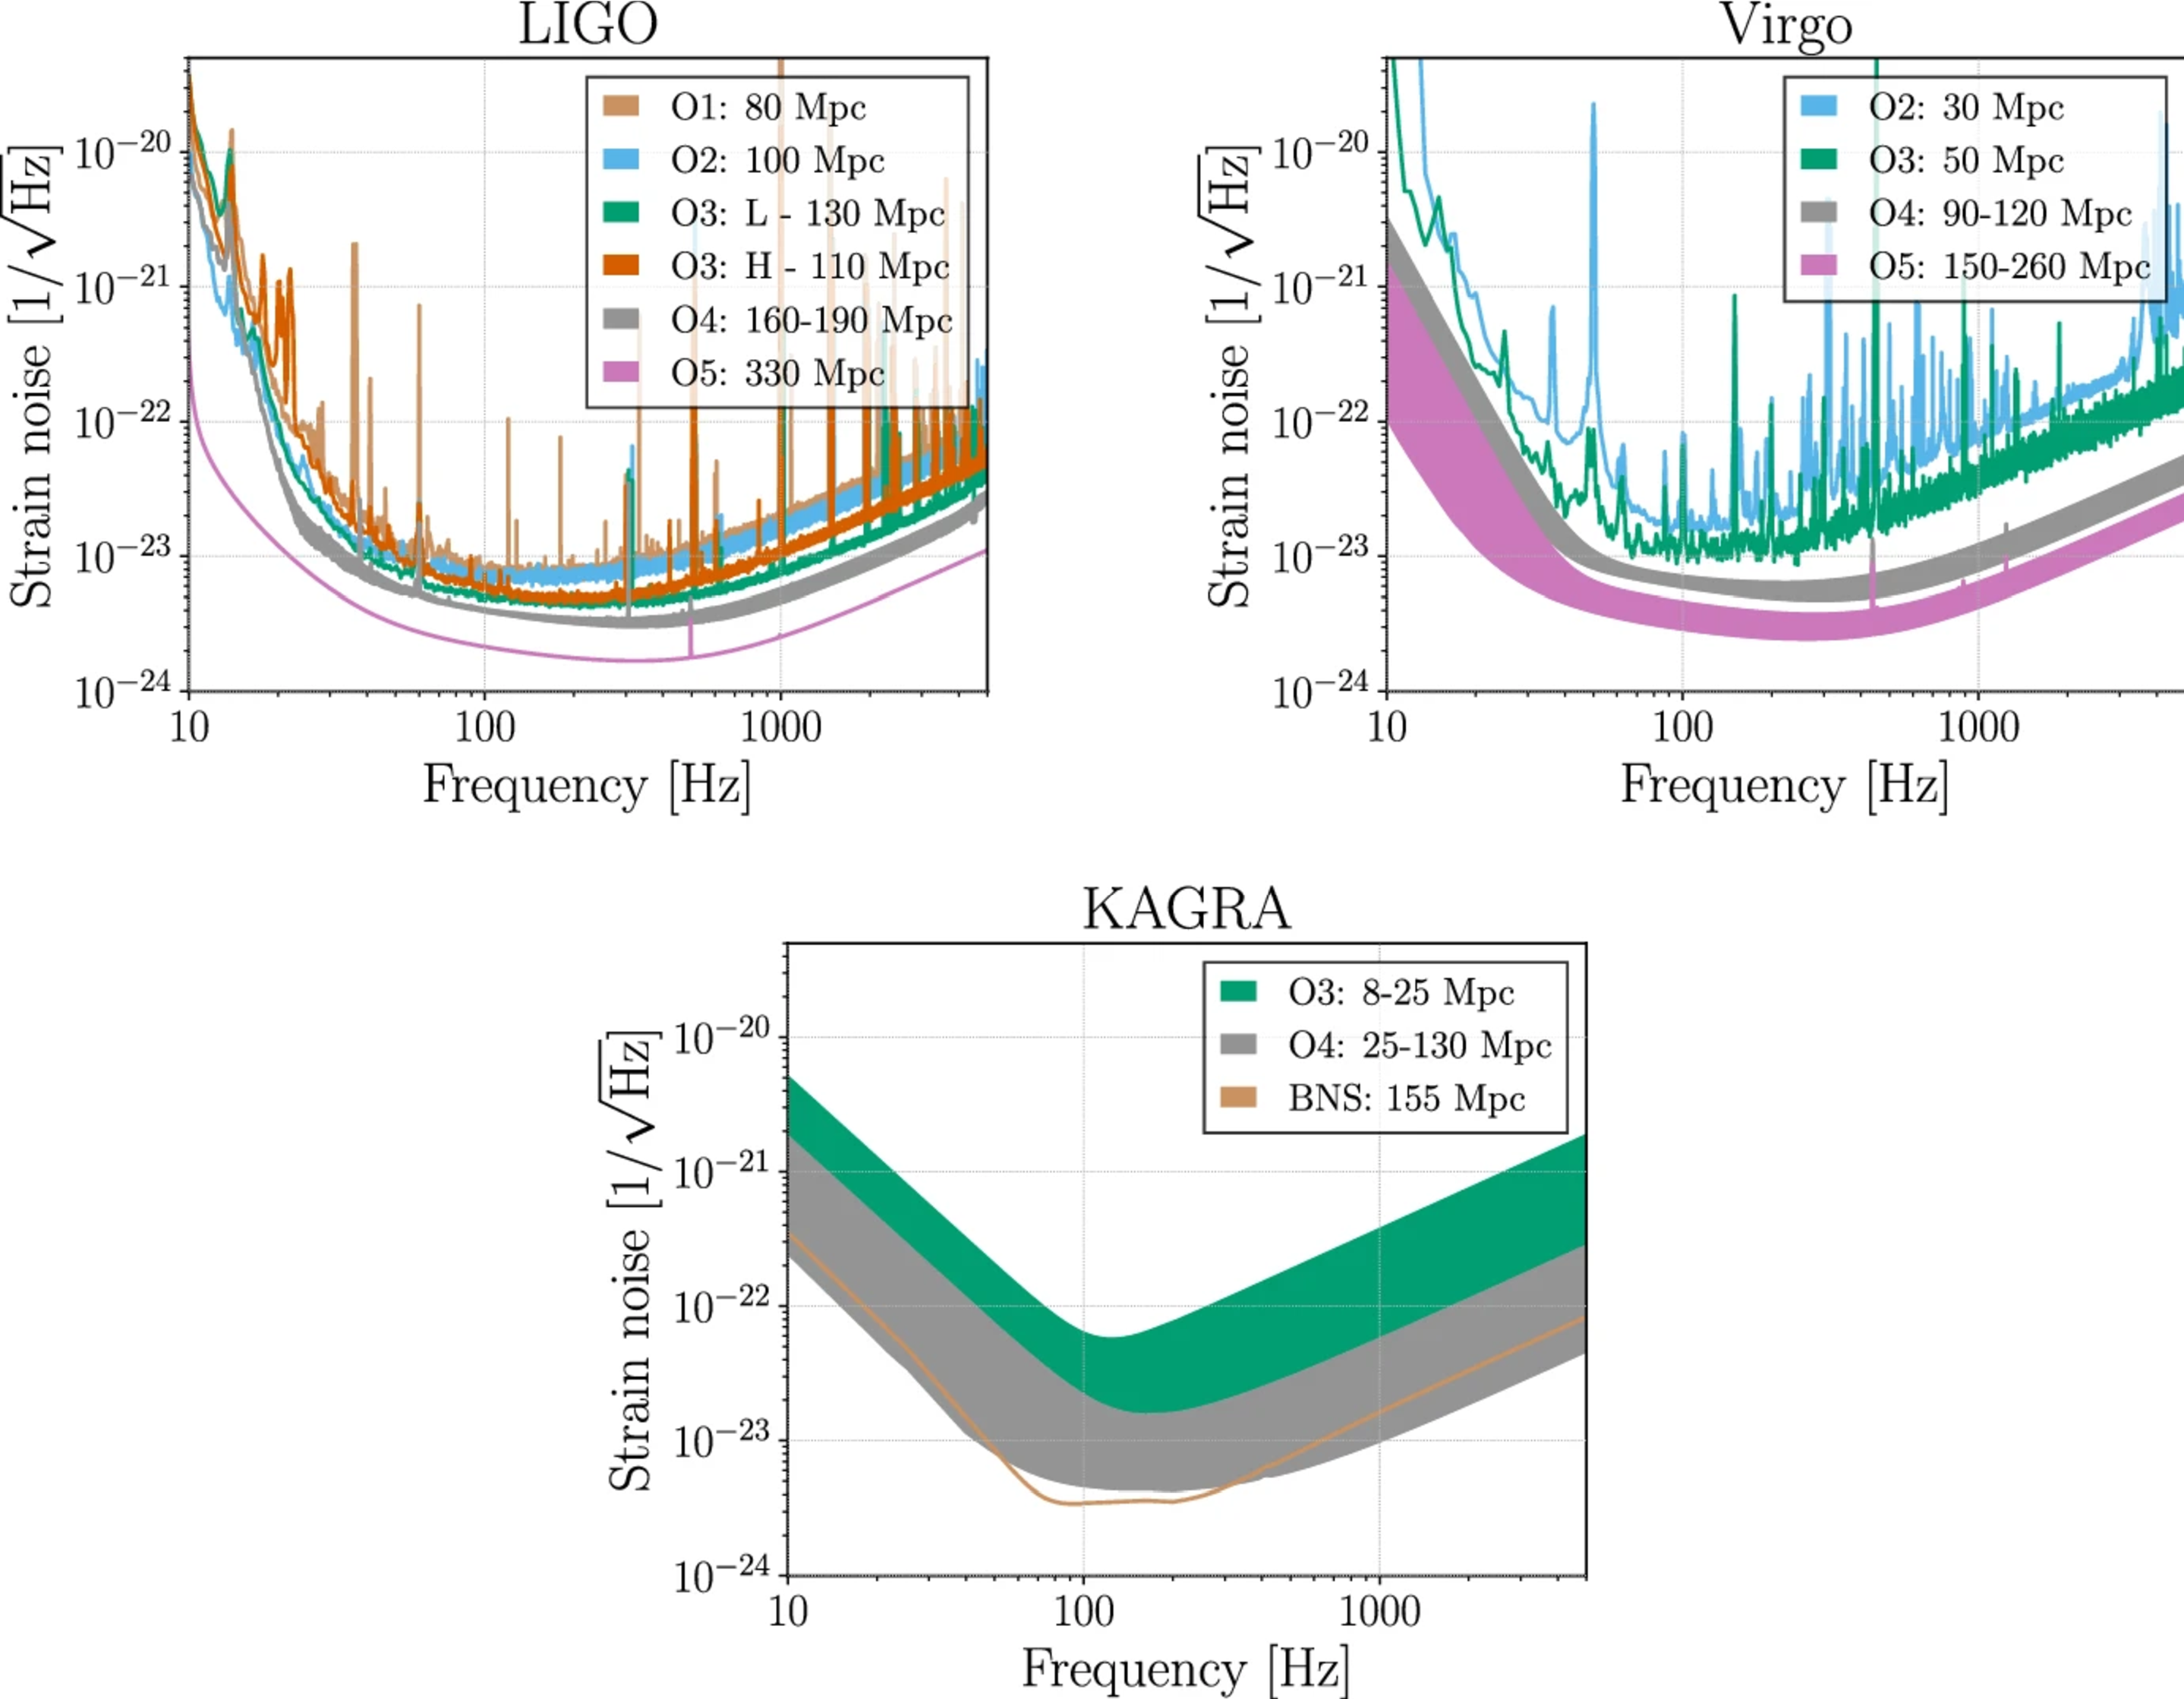
\includegraphics[width=0.3\textwidth]{figures/Capitolo_3/noiseO4.pdf}
%	\end{center}
%	\vspace{-5pt}
%	\caption{Sensibilità del network}
%	\label{fig:sensitivity_O4}
%	\vspace{-10pt}
%\end{wrapfigure}
Verrà presentata in questo capitolo un'analisi basata su un grande numero di forme d'onda iniettate in posizioni celesti generiche e ricostruite con cWB. Nella prima parte verrà fatta l'analisi delle curve di sensibilità e degli overlap, mentre la seconda parte sarà un'analisi volta a stimare sistematicamente la frequenza del post-merger, in particolare utilizzato sulle EOS APR4 e SHT2.
Le simulazioni utilizzano stime intermedie per le sensibilità che raggiungerà il network LIGO-Virgo nel run O4, non si considera invece il detector Kagra, nonostante sia previsto il suo utilizzo ben prima.

\section{Esempi di analisi utilizzando cWB}
\label{section:examples}
Vengono ora riportati alcuni esempi di analisi di eventi simulati utilizzando cWB, partendo da forme d'onda simulate a partire da due diverse EOS. 
%In particolare per ogni analisi verranno riportati i seguenti grafici e coefficienti:
%\begin{itemize}
%		\item il 
%		\item i grafici dell'ampiezza di strain ricostruita nel dominio dei tempi e nel dominio delle frequenze relative a un solo rivelatore.		
%\end{itemize}
\subsection{Equazione di stato APR4}
\label{subsection:APR4}
\begin{minipage}[c]{0.55\textwidth}
	Si riportano i principali coefficienti per identificare l'evento: il rapporto segnale su rumore (SNR); il valore del coefficiente $\rho$, ovvero una ranking statistic che esprime la significanza del segnale descrivendo l'ampiezza correlata effettiva; il coefficiente $c_{net}$ descritto in equazione \ref{eqn:coefficient_energy}; ED che descrive lo sbilanciamento dell'energia tra i detector nel network e, infine, $\theta$ e $\phi$ che descrivono la posizione celeste della sorgente;
\end{minipage}
\hspace{5mm}
\begin{tabular}{cccccc}
	\toprule
	SNR	&$\rho$	&$c_{net}$	&ED	&$\theta$	&$\phi$	\\
	\midrule
	103.1	&50.8	&0.97	&-0.1	&101.6	&-28.6	\\
	\bottomrule
\end{tabular}
\begin{figure}[H]
	\vspace{-20pt}
	\centering
	\subfloat[][\emph{LIGO-Livingstone}]
	{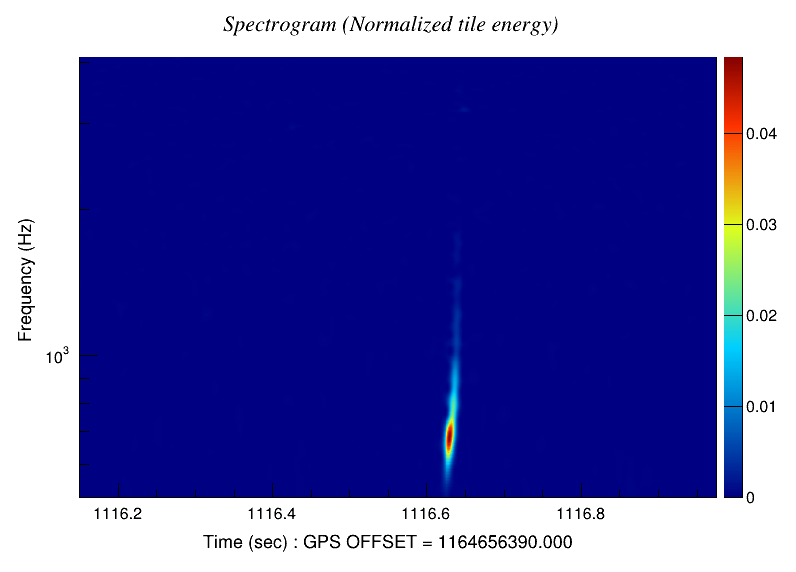
\includegraphics[width=.318125\textwidth]{figures/Capitolo_3/APR4_q09/L1_spectrogram_logy_0.png}} \quad
	\subfloat[][\emph{LIGO-Hanford}]
	{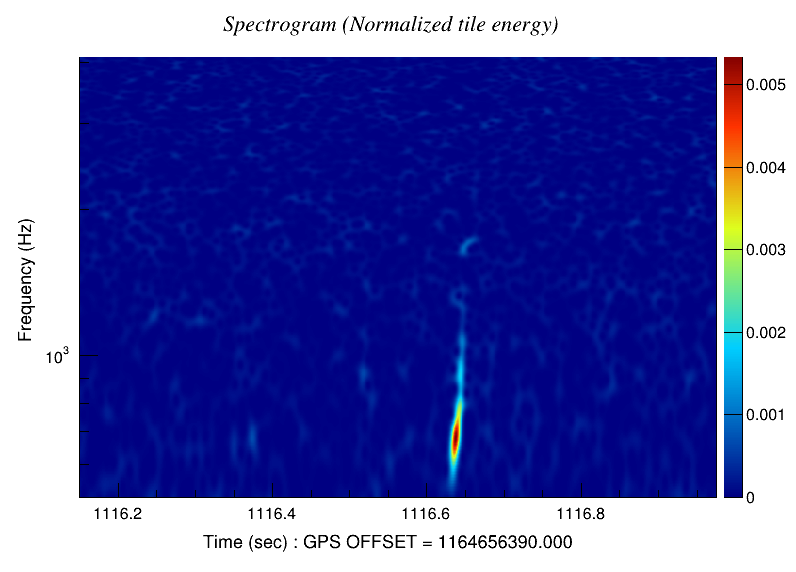
\includegraphics[width=.318125\textwidth]{figures/Capitolo_3/APR4_q09/H1_spectrogram_logy_0.png}} \quad
	\subfloat[][\emph{Virgo}]
	{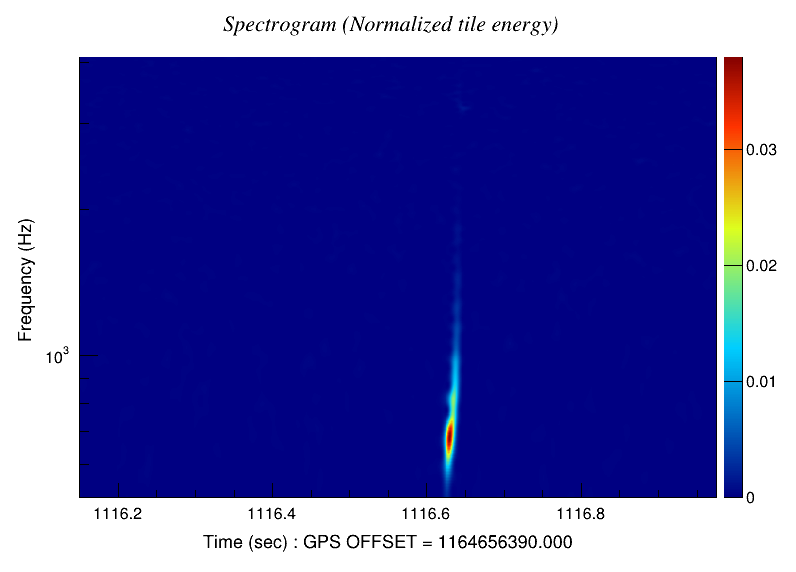
\includegraphics[width=.318125\textwidth]{figures/Capitolo_3/APR4_q09/V1_spectrogram_logy_0.png}}
	\vspace{-5pt}
	\caption{Spettrogrammi per ciascun detector, che mostrano una rappresentazione sul piano tempo-frequenza del trigger, basandosi sulla scomposizione di Fourier}
	\label{fig:spettrogramma_apr4}
	\vspace{-15pt}
\end{figure}
Il segnale che si mostra è particolarmente energetico, perché è stato simulato ad una distanza molto ravvicinata ($d \simeq 1.25$Mpc). Si osservano quindi coefficienti particolarmente elevati.
Come si può osservare in Figura \ref{fig:spettrogramma_apr4}, mentre i detector LIGO-Livingstone e LIGO-Handford rivelano in modo evidente un segnale già ad un'analisi visiva, senza rumore significativo a sporcare la rivelazione, nella mappa di Virgo risulta distinguibile il segnale, tuttavia con rumore significativo e si può notare anche come guardando la scala di significanze del segnale questo risulti di un ordine di grandezza inferiore per Virgo, rispetto ai due rivelatori LIGO. Questo è probabilmente dovuto al fatto che i rivelatori LIGO sono allineati tra loro, mentre disallineati rispetto a Virgo e soprattutto alla posizione celeste della sorgente, favorevole ai primi due.

\begin{wrapfigure}{r}{0.46\textwidth}
	\vspace{-35pt}
	\begin{center}
		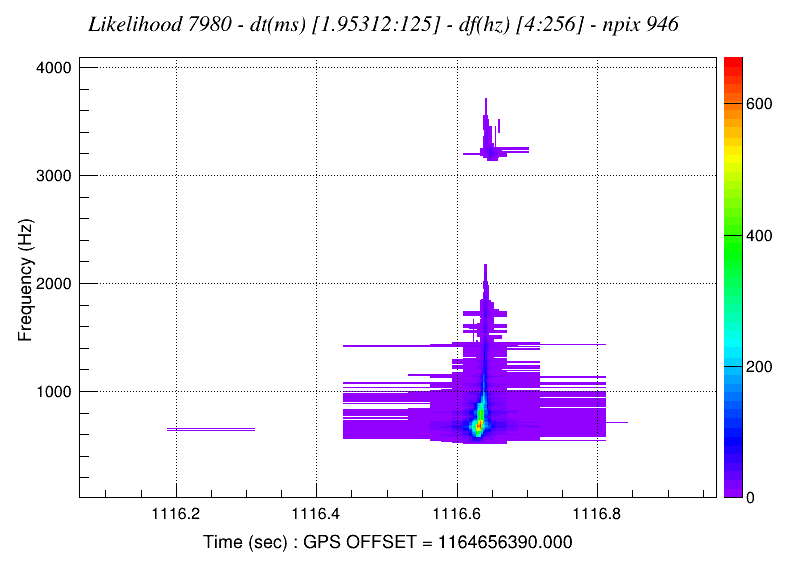
\includegraphics[width=0.475\textwidth]{figures/Capitolo_3/APR4_q09/l_tfmap_scalogram.png}
	\end{center}
	\vspace{-5pt}
	\caption{Mappa di verosimiglianza nel piano tempo-frequenza, che descrive il contributo dell'energia totale del campione associato all'evento ricostruito}
	\label{fig:Likelihood_APR4}
	\vspace{-10pt}
\end{wrapfigure}
Nel grafico della likelihood in figura \ref{fig:Likelihood_APR4}, si osserva una tipica figura a chirp, in cui la parte inferiore, a basse frequenze, rappresenta l'inspiral fino alla coalescenza, mentre il cluster di dati in alto, a frequenze particolarmente elevate ($\smallsim 3.3$KHz) corrisponde all'emissione del post-merger.
Infine nei grafici che seguono in figura \ref{fig:strain_apr4} si osservano le ricostruzioni della forma d'onda, in particolare in nero è plottato il segnale iniettato nella simulazione, mentre in rosso il segnale ricostruito. In particolare osservando il grafico delle frequenze si può notare come non sia stato ricostruito tra $\smallsim2.5$KHz e $\smallsim3$KHz, giustificando la separazione tra i cluster nel grafico della likelihood.
\begin{figure}[H]
	\vspace{-20pt}
	\centering
	\subfloat[][\emph{Dominio dei tempi}]
	{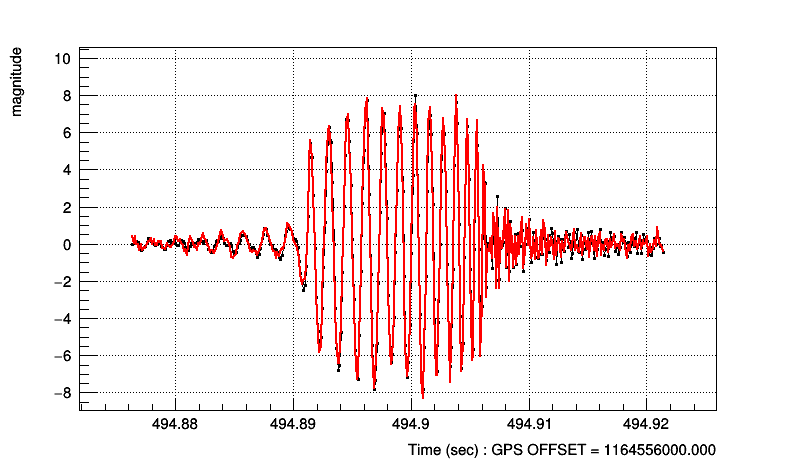
\includegraphics[width=.45\textwidth]{figures/Capitolo_3/APR4_q09/L1_wf_white_inj_rec.png}} \quad
	\subfloat[][\emph{Dominio delle frequenze}]
	{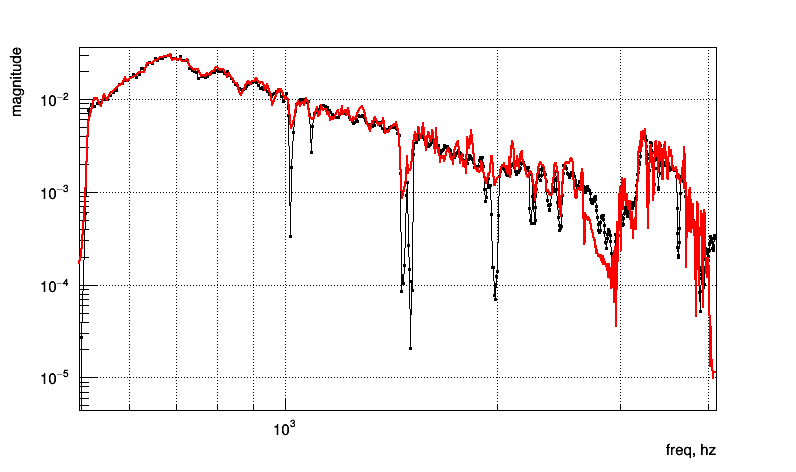
\includegraphics[width=.45\textwidth]{figures/Capitolo_3/APR4_q09/L1_wf_white_inj_rec_fft.png}}
	\vspace{-5pt}
	\caption{Ampiezza di strain ricostruita nel dominio dei tempi e nel dominio delle frequenze relative a un solo rivelatore}
	\label{fig:strain_apr4}
	\vspace{-15pt}
\end{figure}
\subsection{Equazione di stato SHT2}
\label{subsection:SHT2}
Per motivi di spazio non verranno presentate le analisi complete, come per l'equazione di stato precedente, ma si mostreranno solo i grafici delle likelihood: le due forme d'onda iniettate differiscono per la massa delle NS per la coalescenza, in particolare nella \ref{fig:likelihood_sht2}(a), con masse tali da andare in ipermassiva, si può notare come sia presente un segnale di post-merger a $\smallsim 2.5$kHz mentre nella \ref{fig:likelihood_sht2}(b), che ha masse tali da andare direttamente in buco nero, non vi è nessun segnale di post-merger ma solo un segnale di merger che arriva ad alte frequenze. 
\begin{figure}[H]
	\vspace{-20pt}
	\centering
	\subfloat[][\emph{SHT2.0}]
	{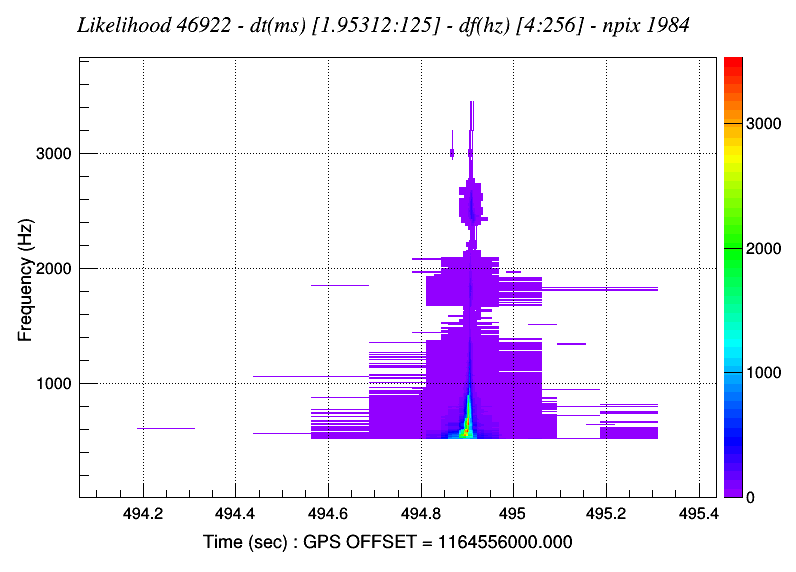
\includegraphics[width=.5\textwidth]{figures/Capitolo_3/SHT2.0spinf1_1/l_tfmap_scalogram.png}}
	\subfloat[][\emph{SHT2.2}]
	{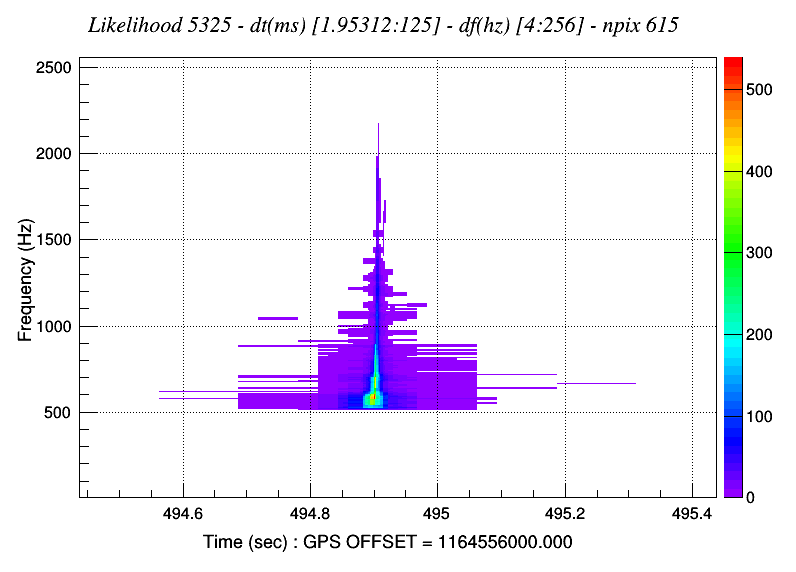
\includegraphics[width=.5\textwidth]{figures/Capitolo_3/SHT2.2spinf1_1/l_tfmap_scalogram.png}}
	\vspace{-5pt}
	\caption{Mappe di verosimiglianza ricostruite per le due forme d'onda iniettate}
	\label{fig:likelihood_sht2}
	\vspace{-15pt}
\end{figure}

\section{Curve di sensibilità e analisi dell'overlap}
\label{section:overlap}
Si riportano gli istogrammi per gli SNR iniettati e ricostruiti dal network, divisi per distanza della sorgente. Si può notare come al crescere della distanza le distribuzioni siano sempre più schiacciate a SNR bassi.
\begin{figure}[H]
	\vspace{-20pt}
	\centering
	\subfloat[][\emph{SHT2.0}]
	{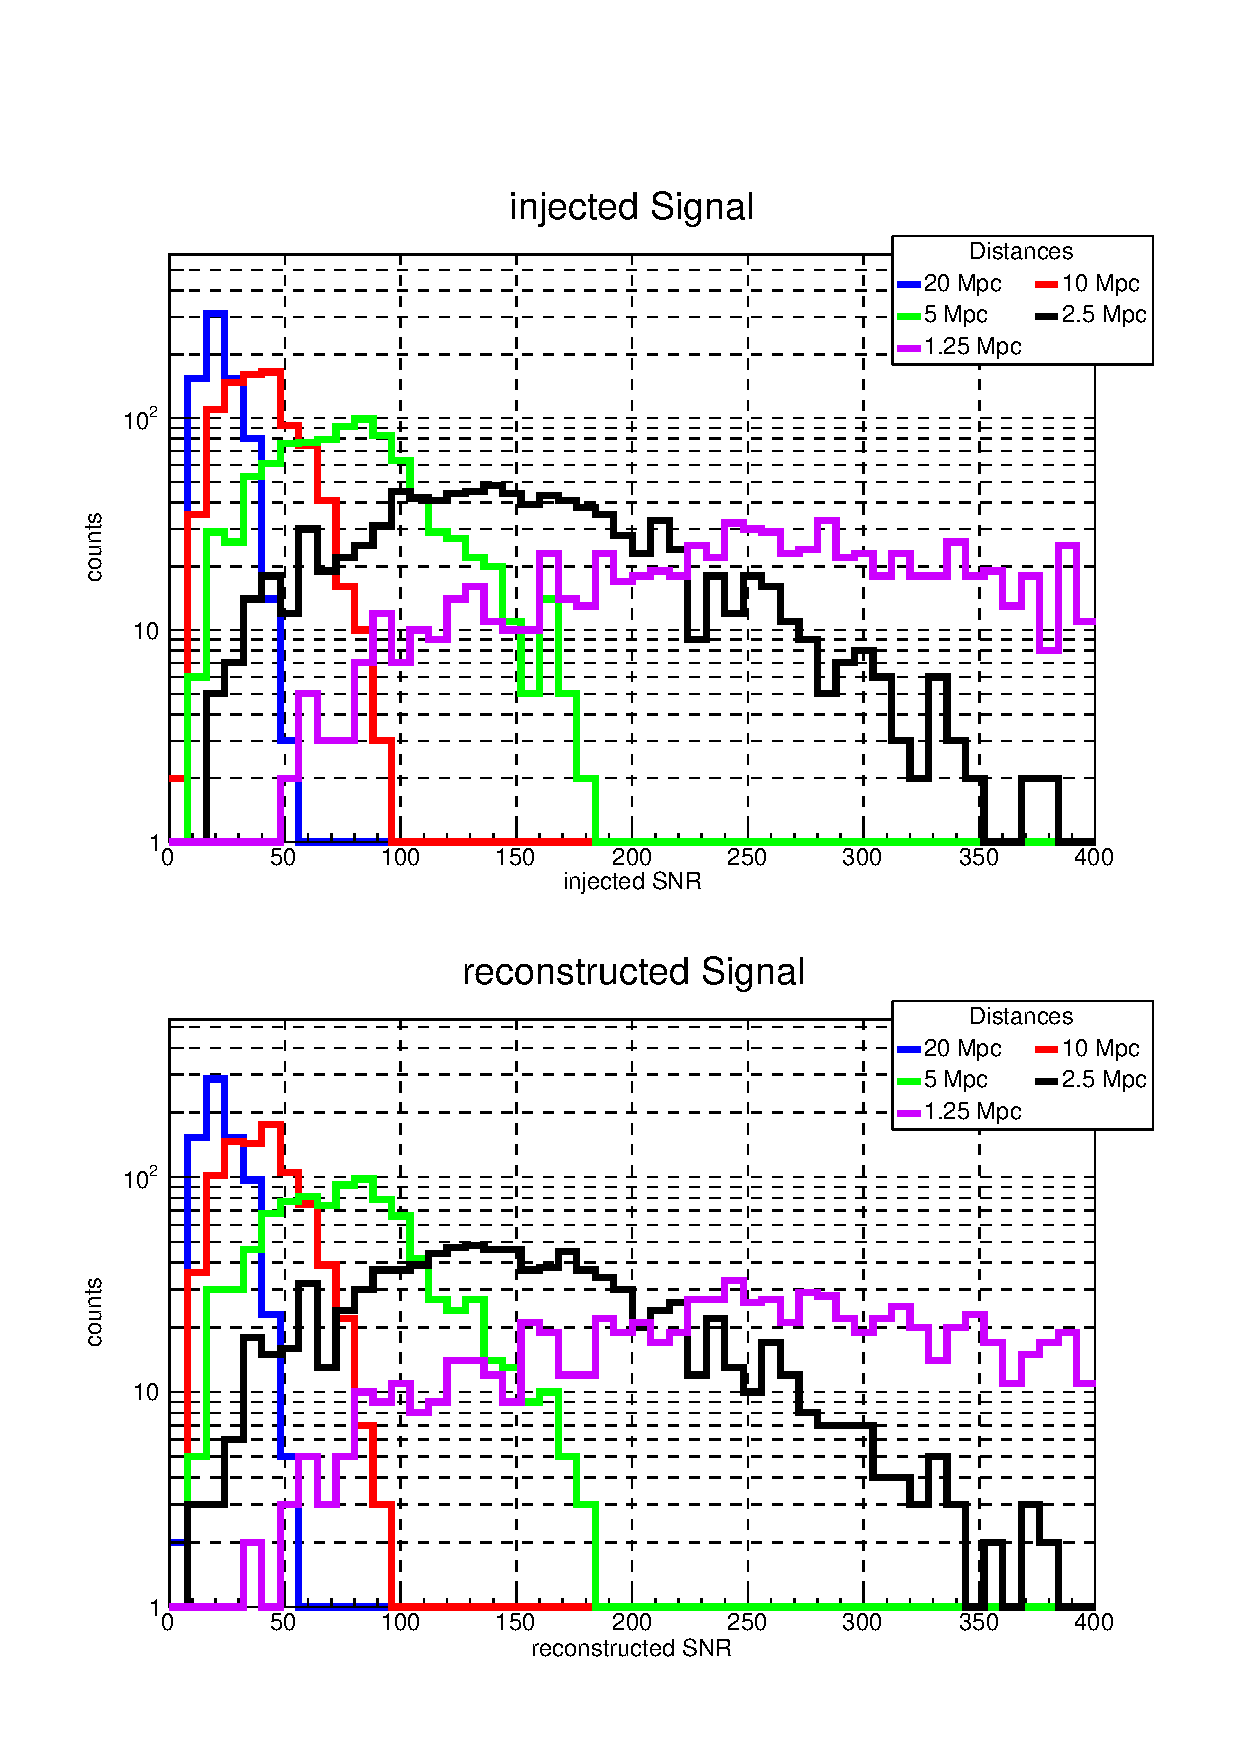
\includegraphics[width=.5\textwidth]{figures/Capitolo_4/Network_SNR_FactorsSHT2_0spin1.pdf}}
	\subfloat[][\emph{APR4}]
	{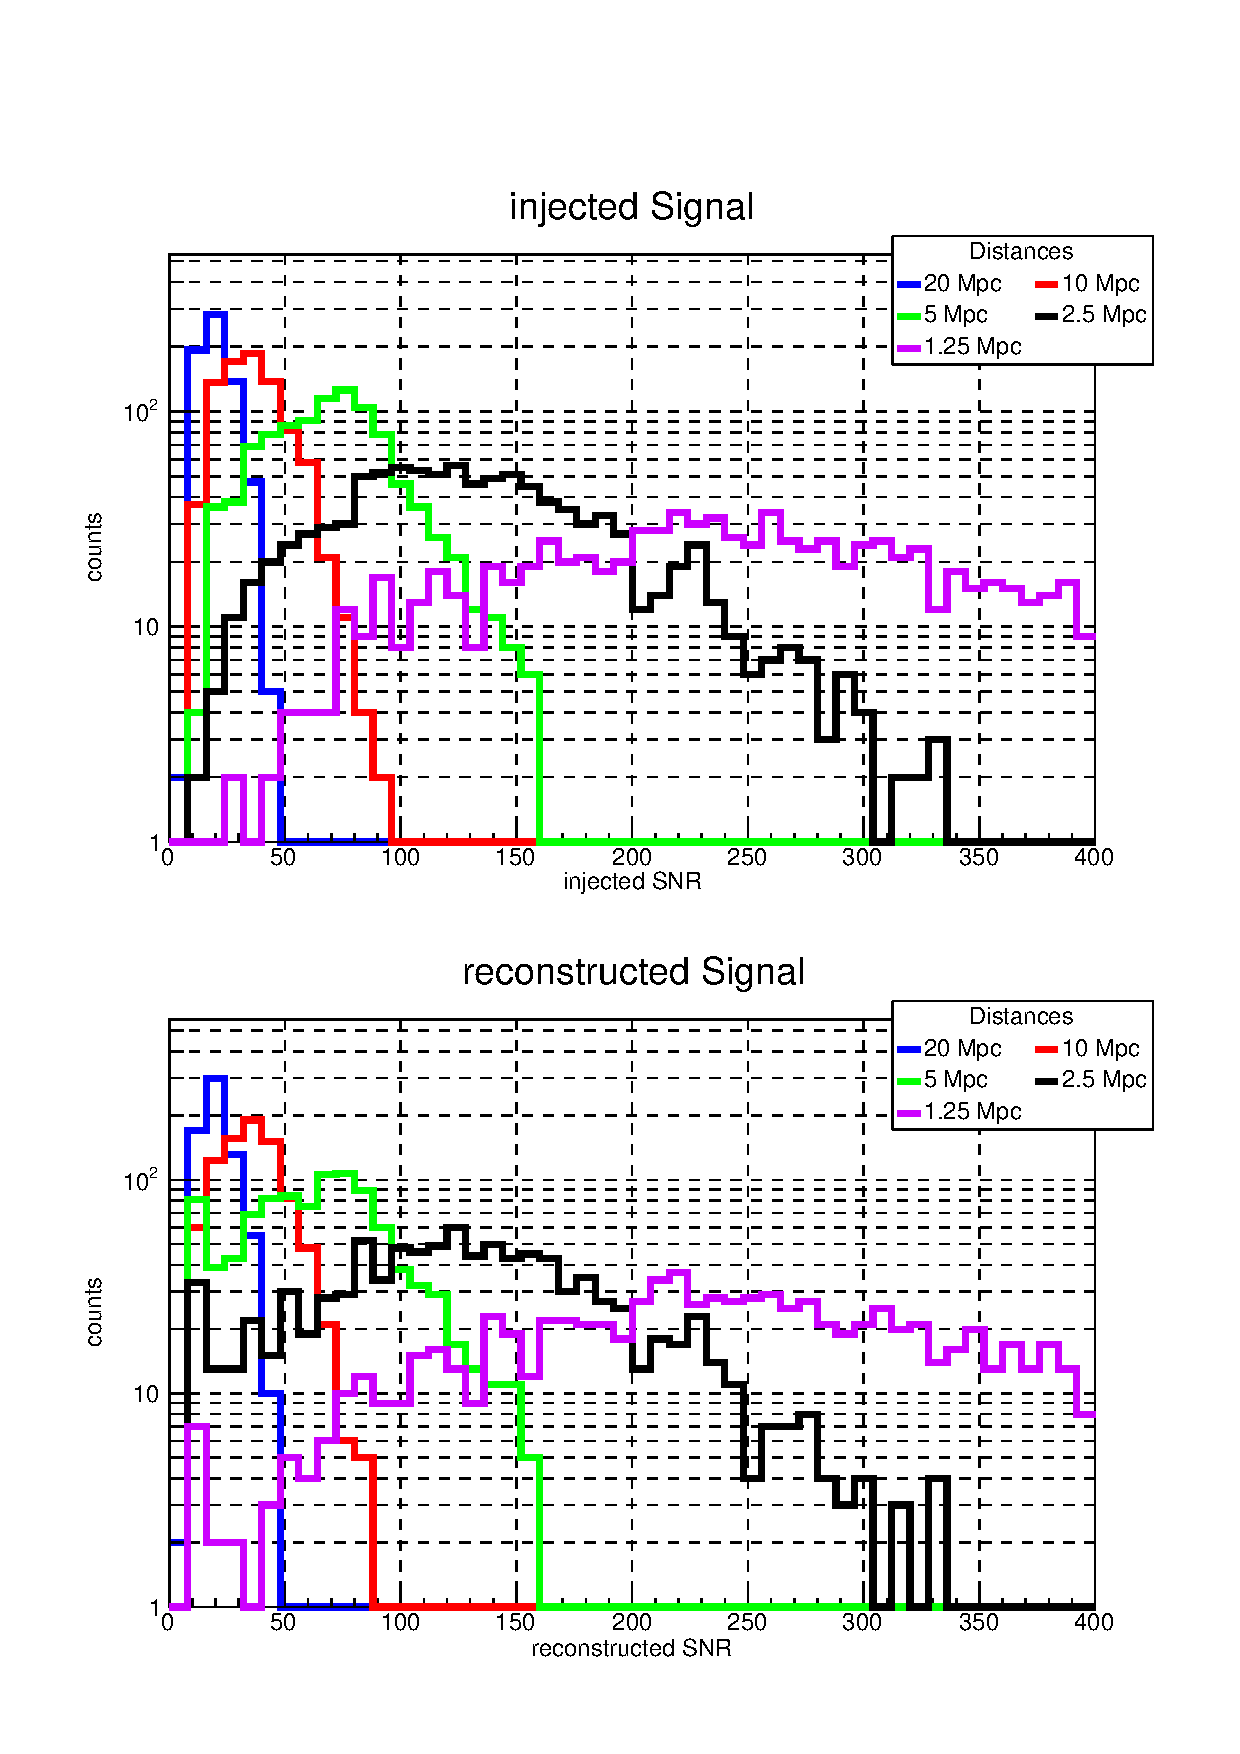
\includegraphics[width=.5\textwidth]{figures/Capitolo_4/Network_SNR_FactorsAPR4_q09.pdf}}
	\vspace{-5pt}
	\caption{SNR iniettato (sopra) e ricostruito (sotto) per le due EOS}
	\label{fig:SNR_INJ_REC_COUNTS}
	\vspace{-15pt}
\end{figure}
Si procede quindi a verificare in modo quantitativo l'efficienza dell'algoritmo di ricostruizione, facendo un fit degli SNR ricostruiti in funzione degli SNR iniettati. L'andamento ideale che ci si aspetta è rappresentato dalla bisettrice del primo e terzo quadrante, che corrisponde a una processo tale per cui l'SNR ricostruito è pari a quello iniettato.
\begin{figure}[H]
	\vspace{-10pt}
	\centering
	\subfloat[][\emph{SHT2}]
	{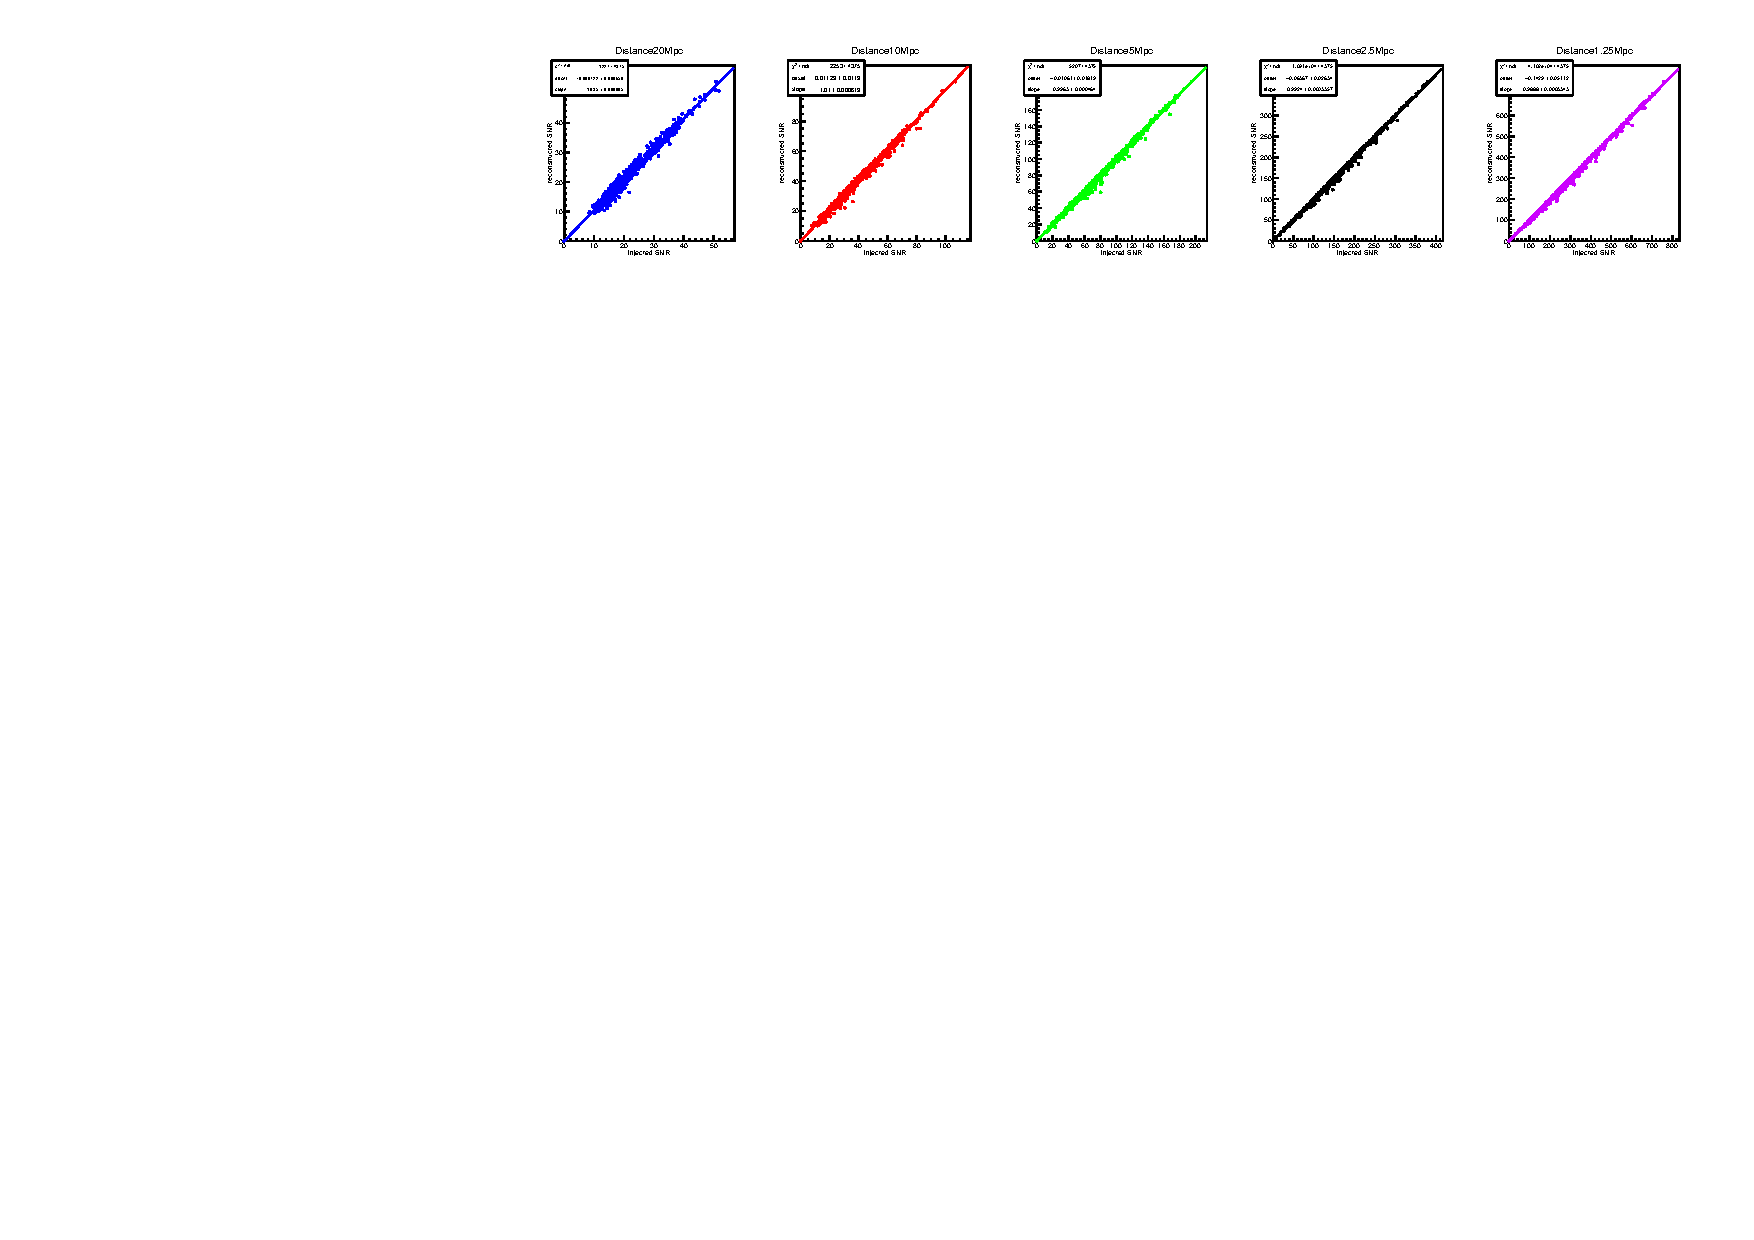
\includegraphics[width=1\textwidth]{figures/Capitolo_4/FITSHT2_0spin1.pdf}} \\
	\vspace{-10pt}
	\subfloat[][\emph{APR4}]
	{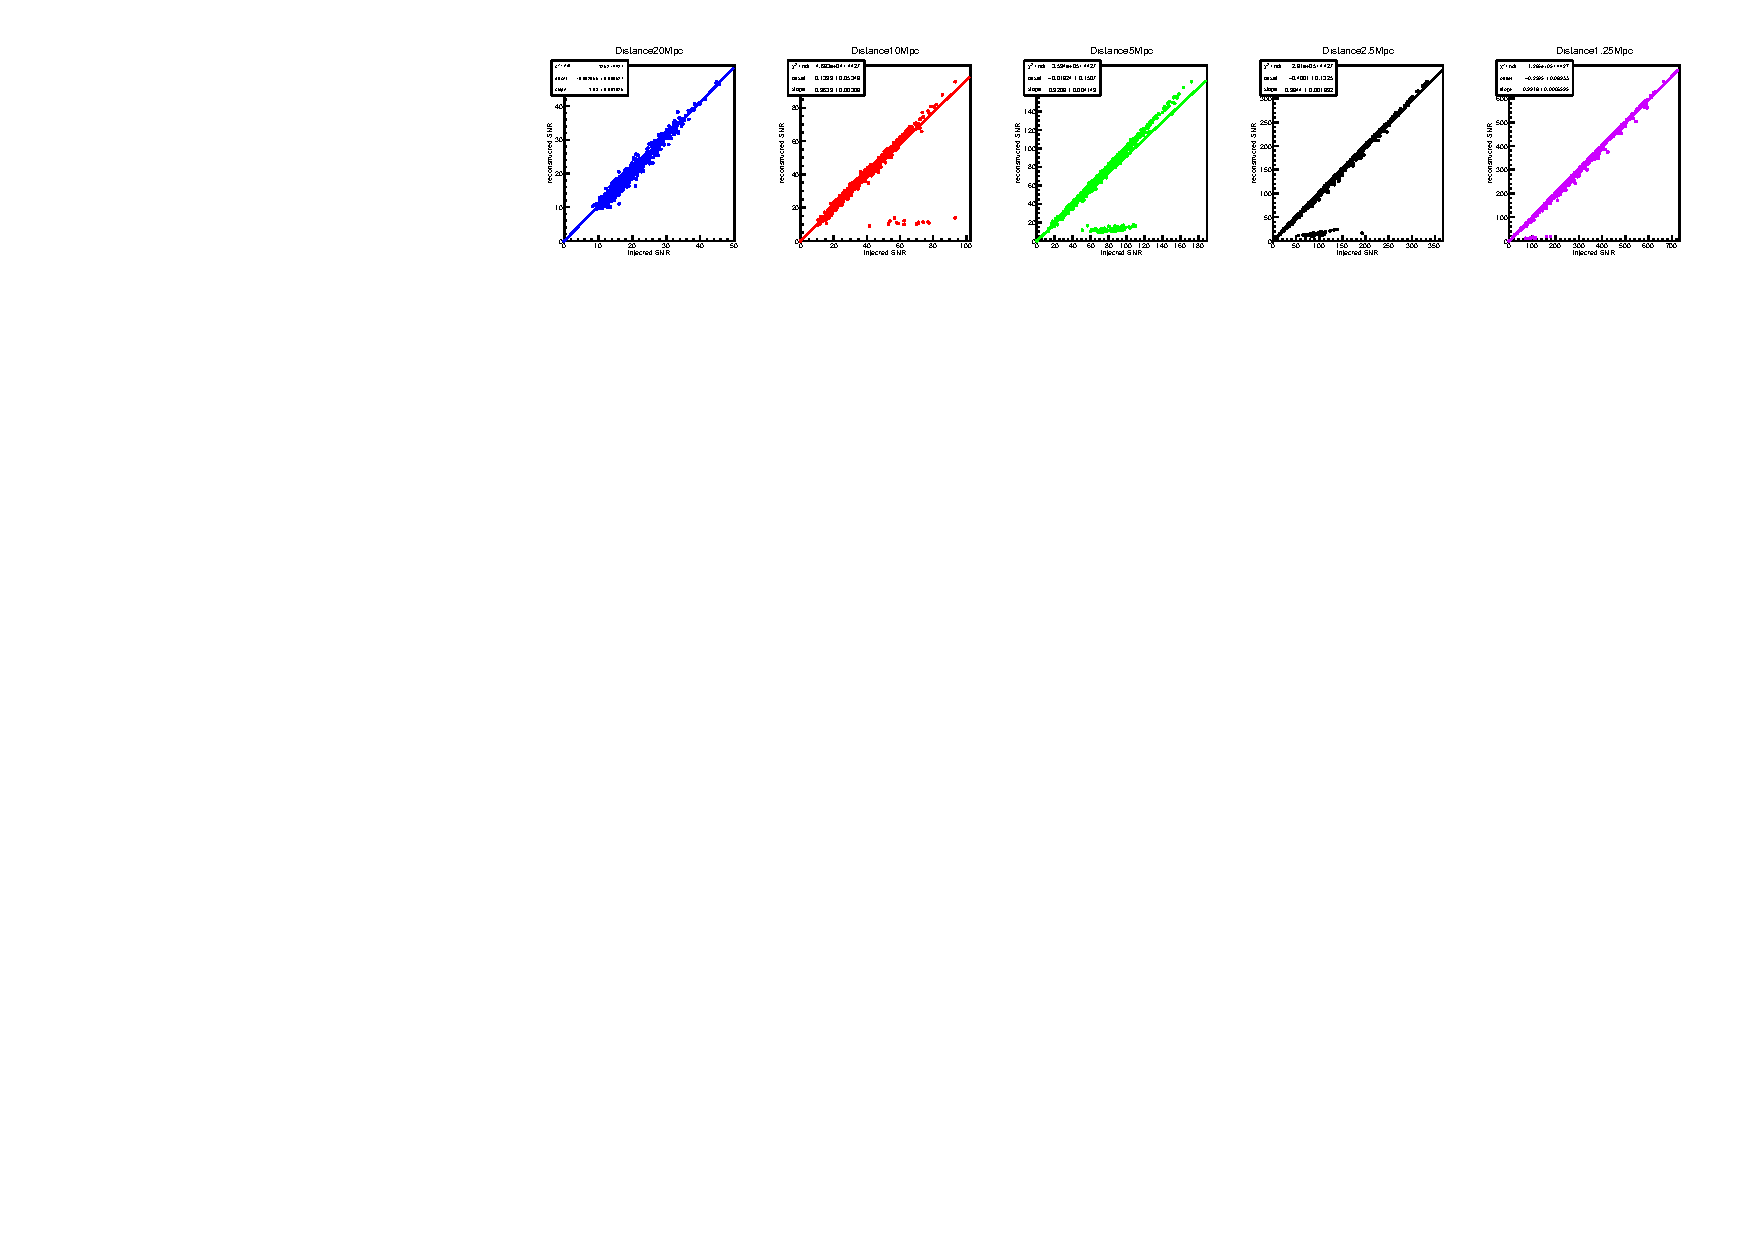
\includegraphics[width=1\textwidth]{figures/Capitolo_4/FITAPR4_q09.pdf}}
	\vspace{-5pt}
	\caption{Fit dell'SNR ricostruito in funzione dell'SNR iniettato per le due EOS}
	\label{fig:overlap}
	\vspace{-15pt}
\end{figure}
Si può notare come, mentre per la EOS SHT2 le ricostruzioni siano ottime e, entro gli errori sperimentali, le rette siano compatibili con l'andamento ideale, per la EOS APR4, in particolare per le distanze intermedie. ci sia un problema nella ricostruzione, che porta ad un fit non compatibile con l'andamento ideale.

Si riportano quindi gli overlap in funzione degli SNR ricostruiti. In particolare si ha che denotando il segnale iniettato e ricostruito per ogni detector come $x_{I}[i]= [x_{I,1}, \dots x_{I,N}]$ e $x_{R}[i]= [x_{R,1}, \dots x_{R,N}]$ rispettivamente, si definiranno allora SNR iniettato e ricostruito come
%\vspace{-25pt}
\begin{equation}
%	\vspace{  -25pt}
	iSNR = \sum_{i=1}^{N}x_{I, i}^2 = |x_{I}|^2 \quad\quad\quad oSNR = \sum_{i=1}^{N}x_{R, i}^2 = |x_{R}|^2
	\label{eqn:iSNR_oSNR}
\end{equation} 
Esiste però un'altra quantità che si ottiene incrociando questi dati definita come $ioSNR = \sum_{i=1}^{N}x_{I, i}x_{R, i}$, ovvero la correlazione incrociata, a ritardo temporale nullo, della forma d'onda iniettata e ricostruita. Grazie a questa quantità è possibile calcolare due grandezze fondamentali: l'energia residua $E_{res}= \sum_{i=1}^{N}(x_{R, i}-x_{I, i})^2 = oSNR + iSNR - 2ioSNR$ e l'$o_{verlap} = \frac{\braket{x_I}{x_R}}{\sqrt{|x_I||x_R|}} = \frac{ioSNR}{\sqrt{|x_I||x_R|}}$ che descrive la corrispondenza del segnale iniettato rispetto a quello ricostruito, in particolare per $o_{verlap}=1$ i due segnali hanno un matching perfetto, per overlap=0 invece non c'è ricostruzione del segnale.
\begin{figure}[H]
	\vspace{-20pt}
	\centering
	\subfloat[][\emph{SHT2}]
	{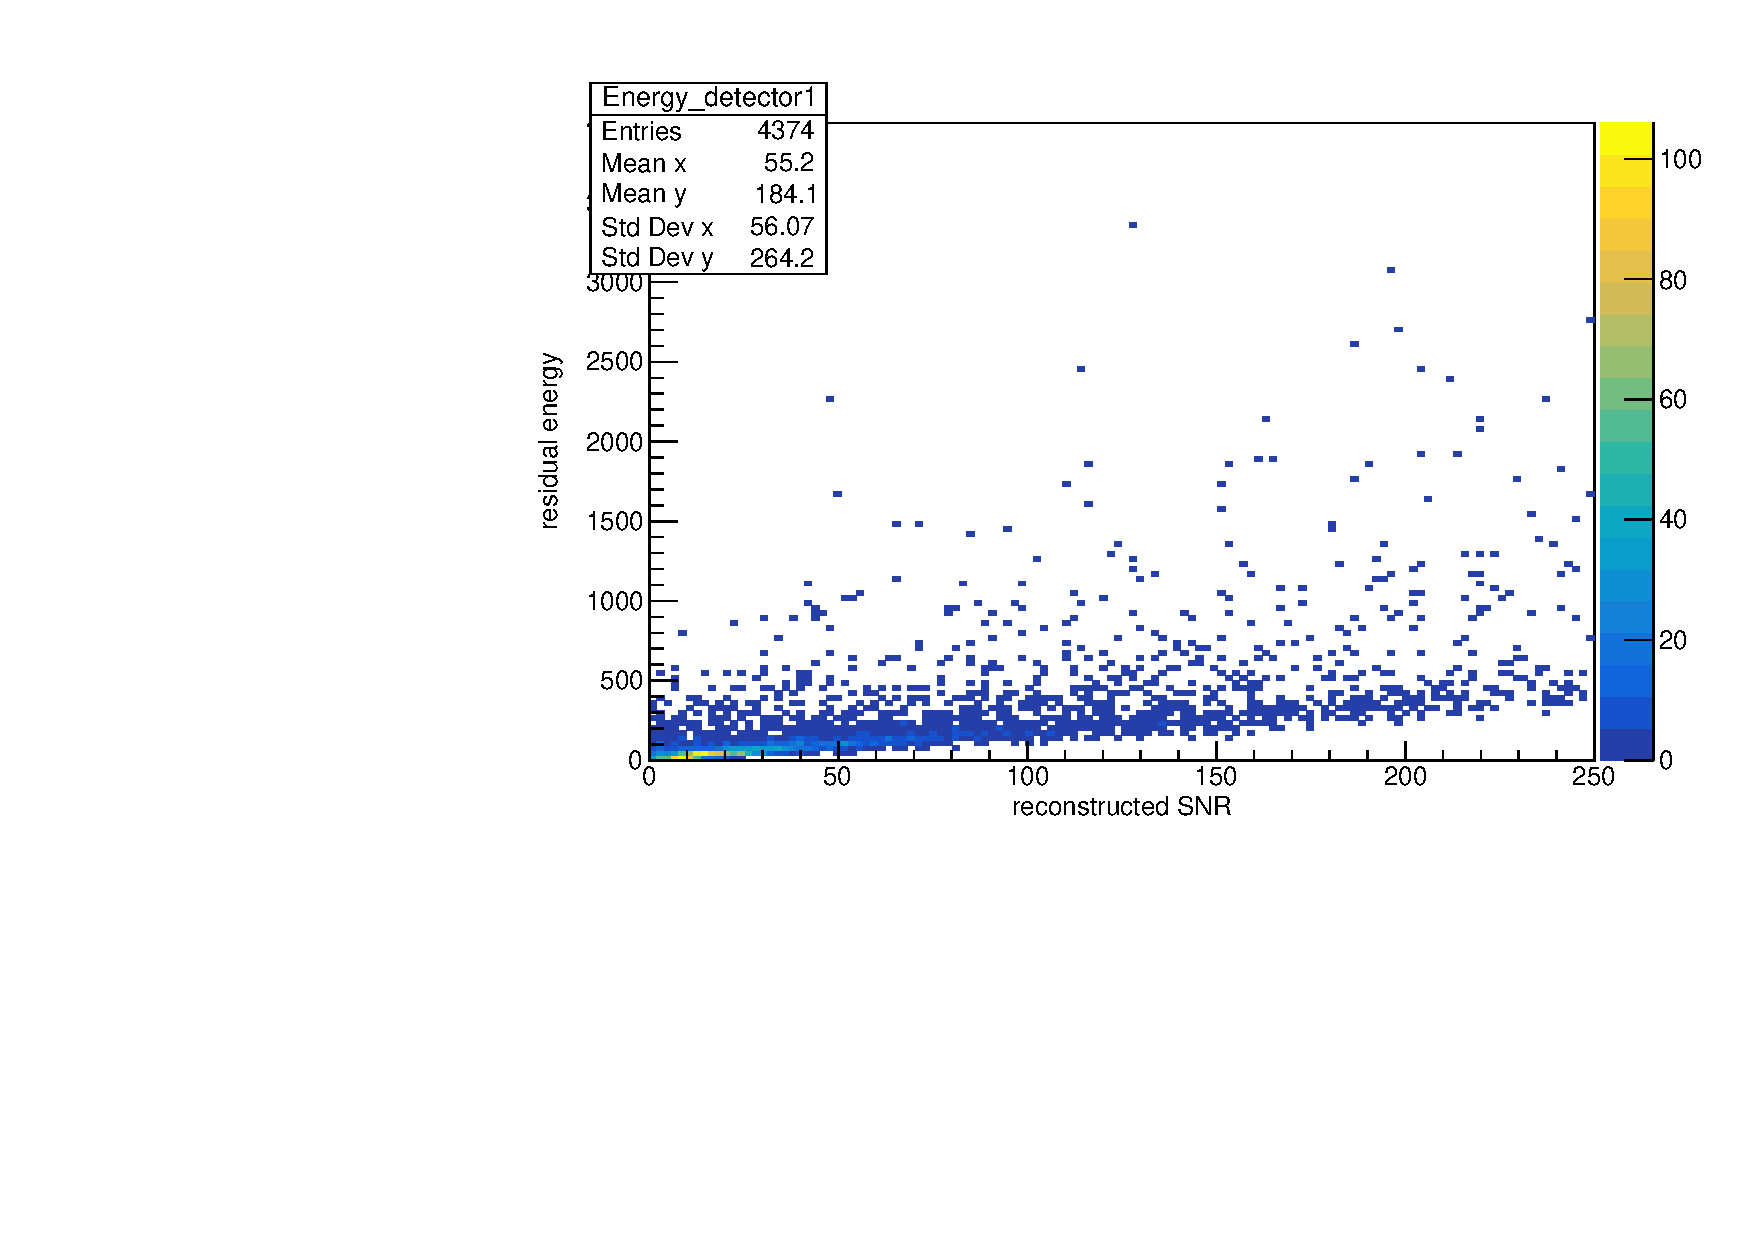
\includegraphics[width=.5\textwidth]{figures/Capitolo_4/EnergyDistributionDetector1SHT2_0spin1.pdf}}
	\subfloat[][\emph{APR4}]
	{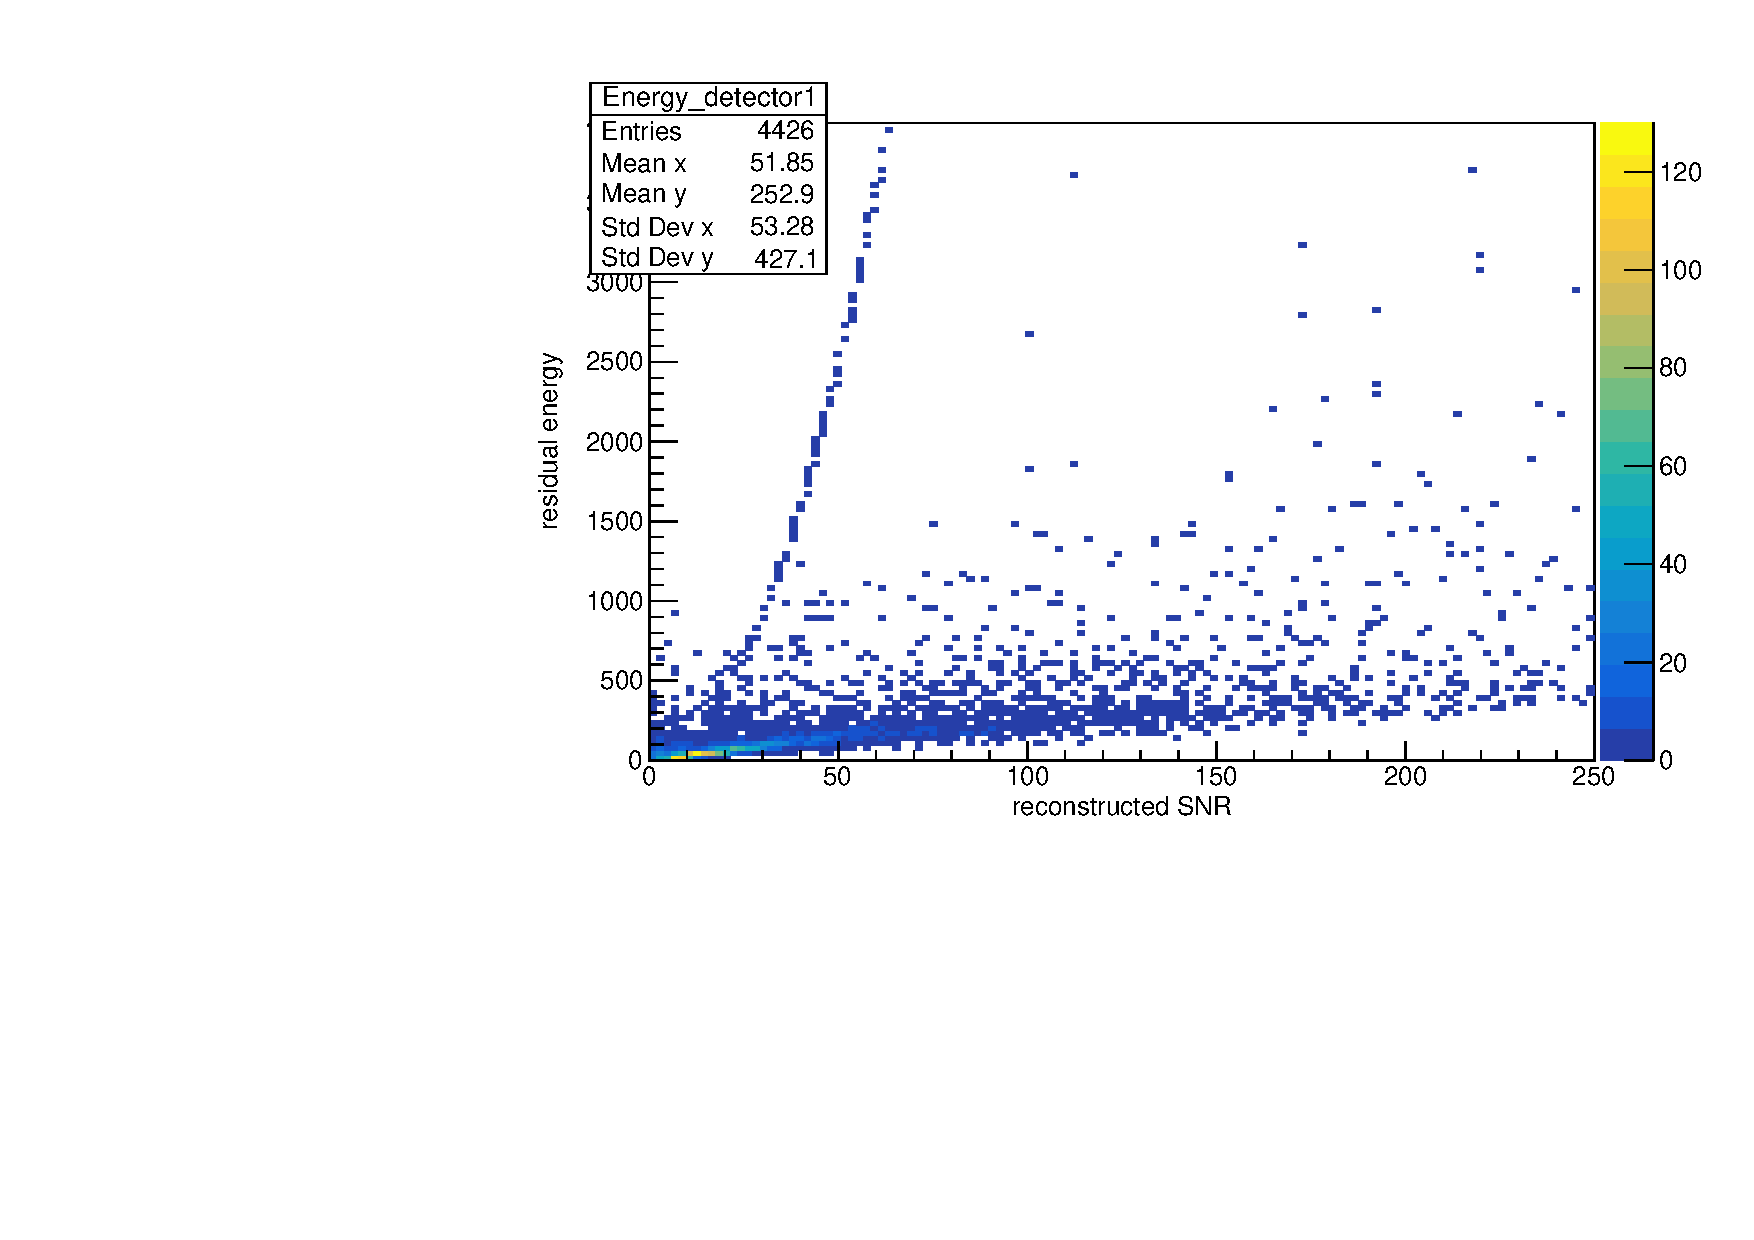
\includegraphics[width=.5\textwidth]{figures/Capitolo_4/EnergyDistributionDetector1APR4_q09.pdf}}
	\vspace{-5pt}
	\caption{Energie residue per LIGO-Hanford per le due equazioni di stato}
	\label{fig:residual_energy}
	\vspace{-15pt}
\end{figure}
\begin{figure}[H]
	\vspace{-17pt}
	\centering
	\subfloat[][\emph{SHT2 per LIGO-Hanford}]
	{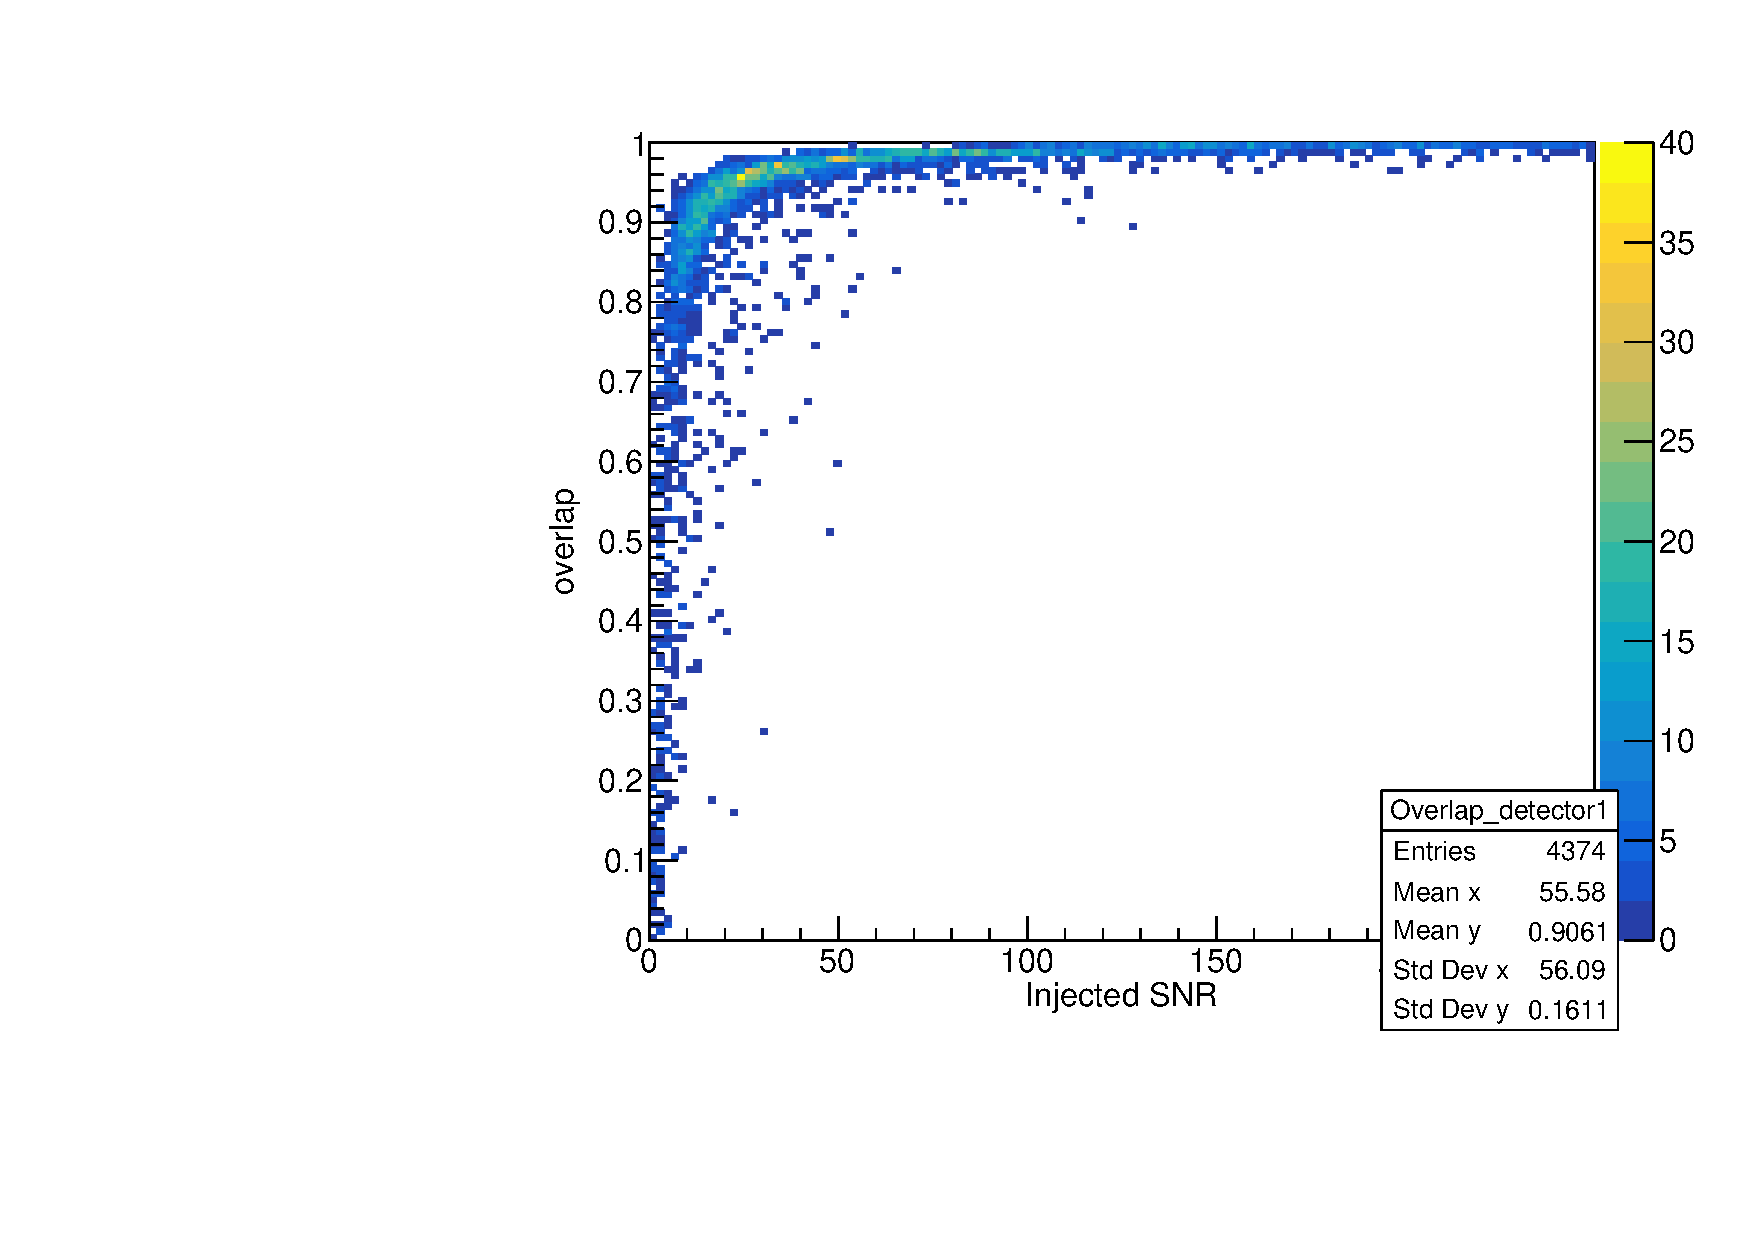
\includegraphics[width=.33\textwidth]{figures/Capitolo_4/OverlapDistributionDetector1SHT2_0spin1.pdf}}% \quad
	\subfloat[][\emph{SHT2 per LIGO-Livingston}]
	{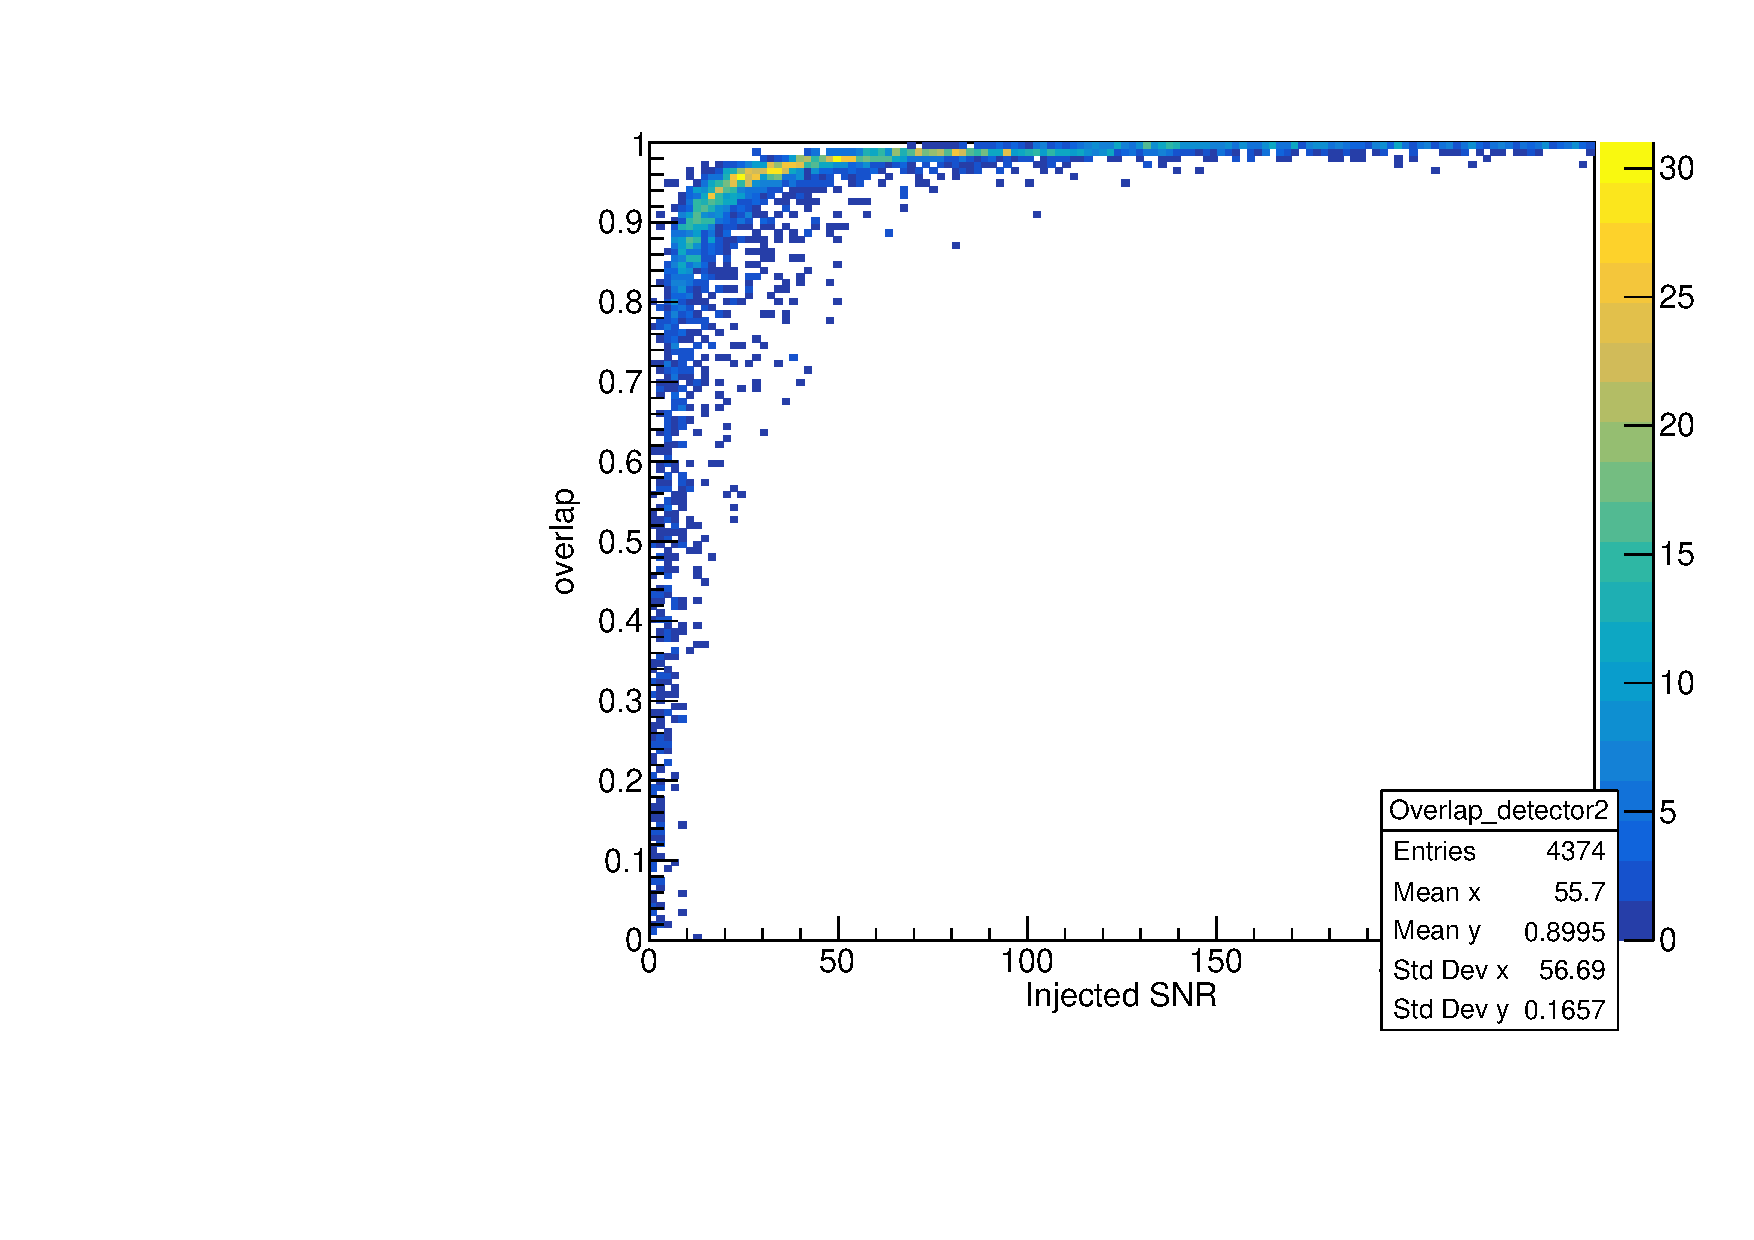
\includegraphics[width=.33\textwidth]{figures/Capitolo_4/OverlapDistributionDetector2SHT2_0spin1.pdf}}%\quad
	\subfloat[][\emph{SHT2 per Virgo}]
	{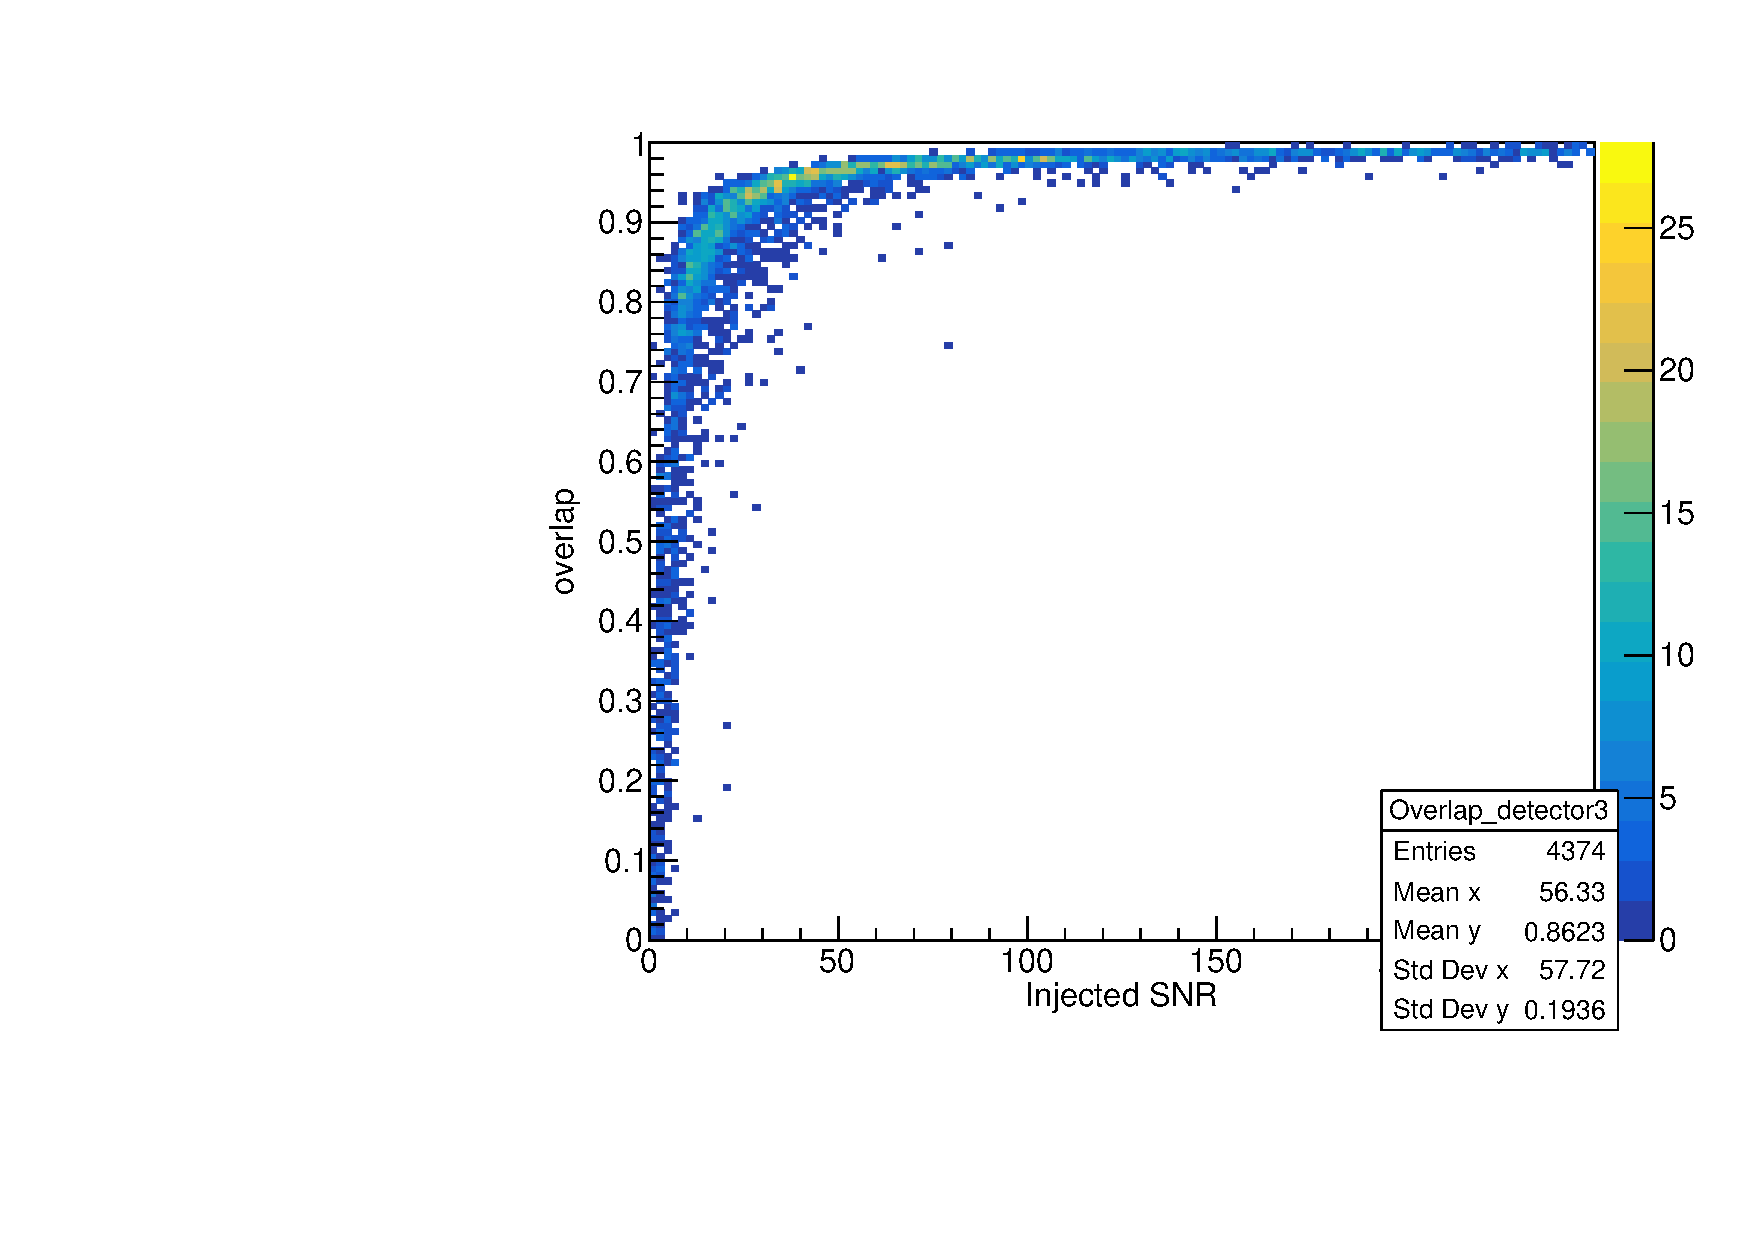
\includegraphics[width=.33\textwidth]{figures/Capitolo_4/OverlapDistributionDetector3SHT2_0spin1.pdf}}\\
	\vspace{-13pt}
	\subfloat[][\emph{APR4 per LIGO-Hanford}]
	{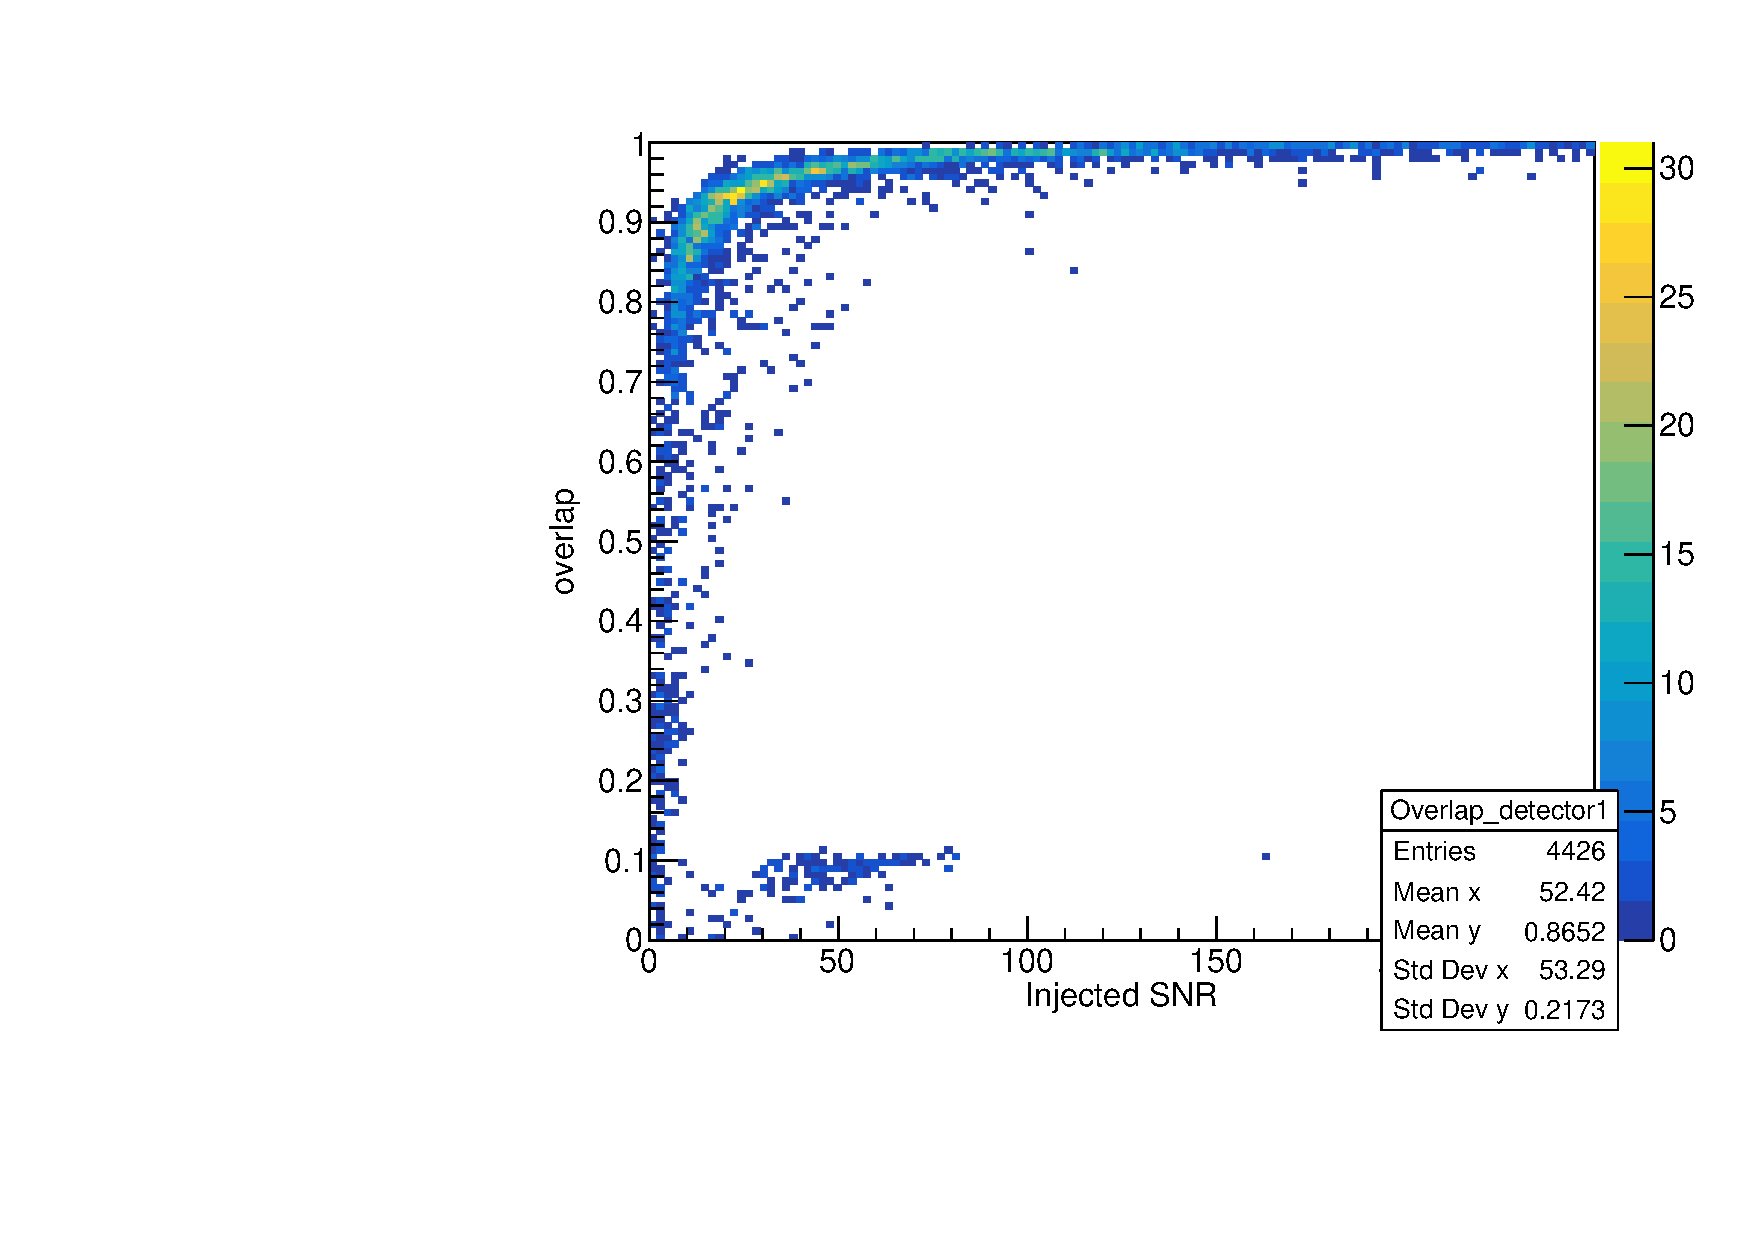
\includegraphics[width=.33\textwidth]{figures/Capitolo_4/OverlapDistributionDetector1APR4_q09.pdf}} %\quad
	\subfloat[][\emph{APR4 per LIGO-Livingston}]
	{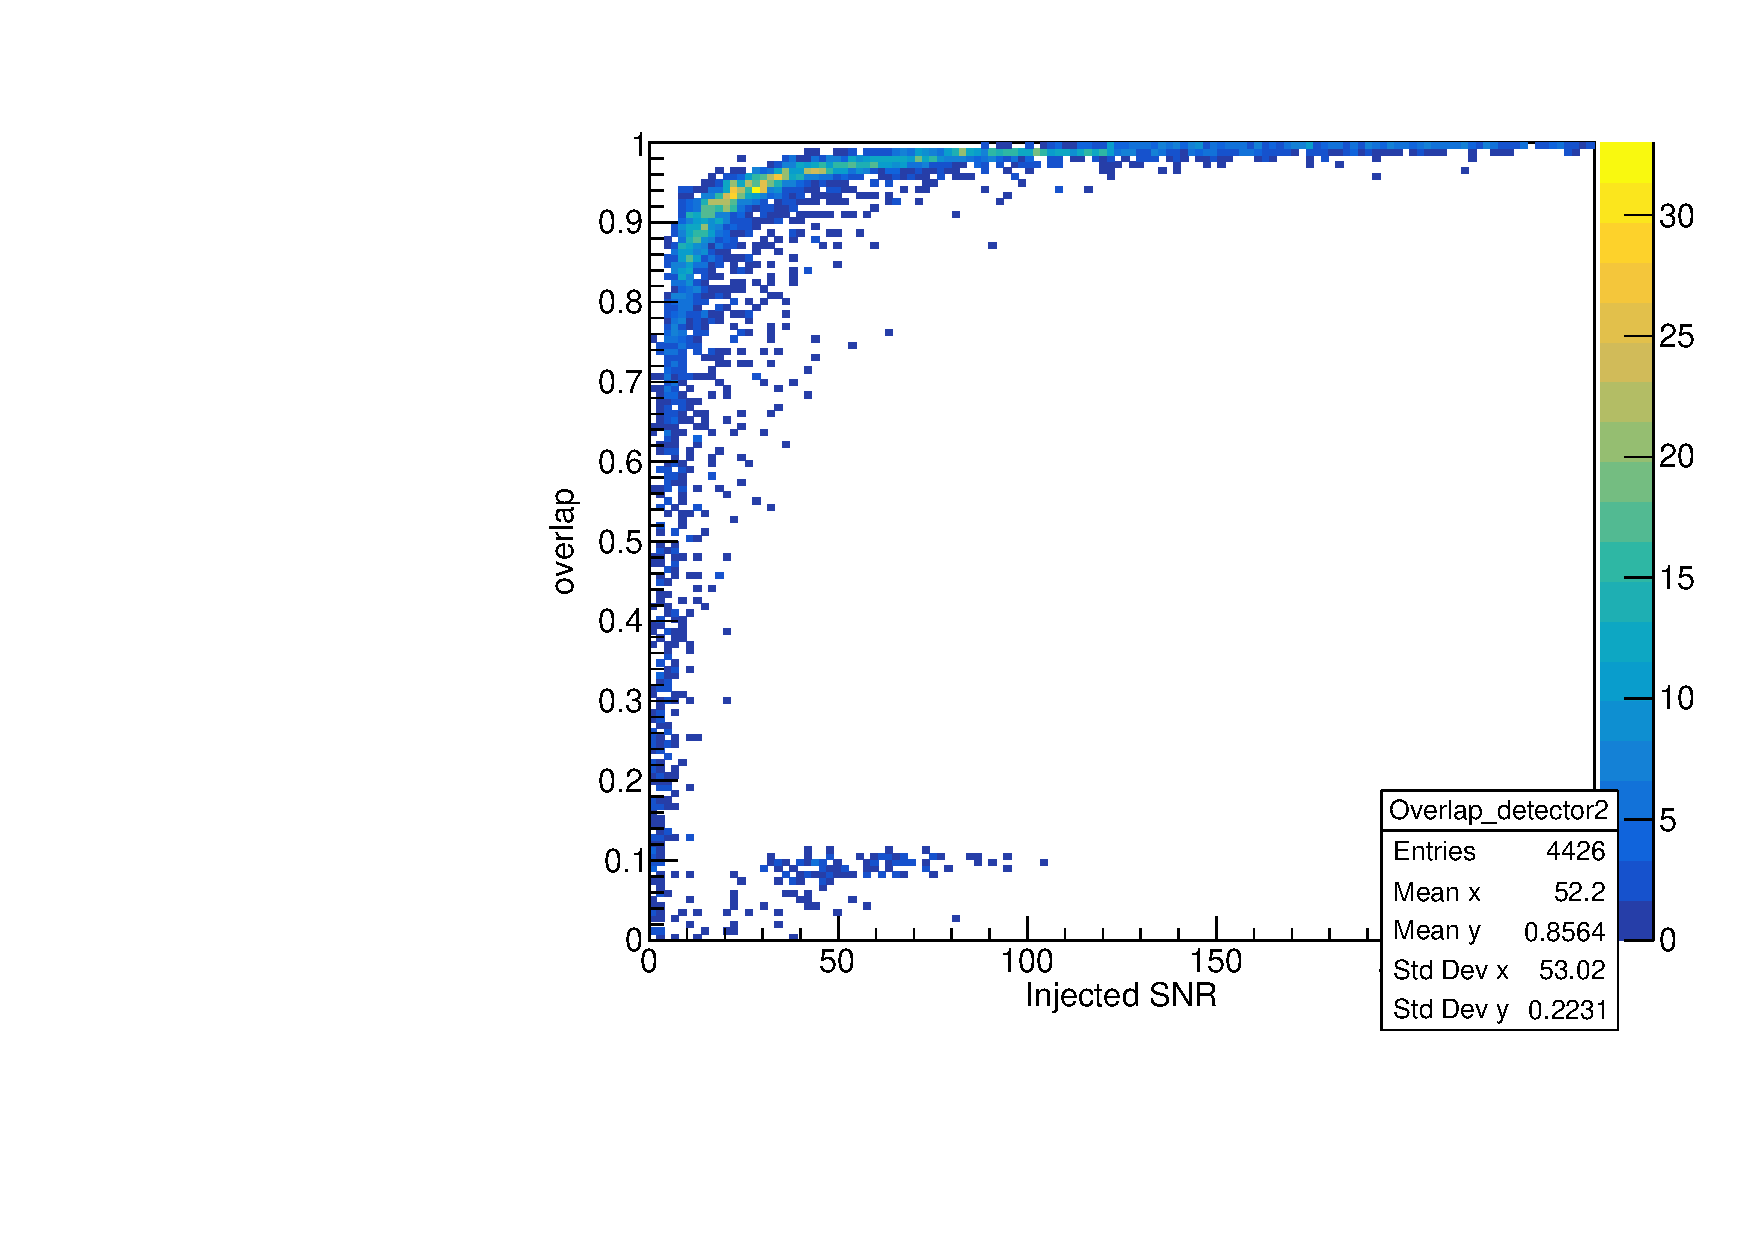
\includegraphics[width=.33\textwidth]{figures/Capitolo_4/OverlapDistributionDetector2APR4_q09.pdf}}%\quad
	\subfloat[][\emph{APR4 per Virgo}]
	{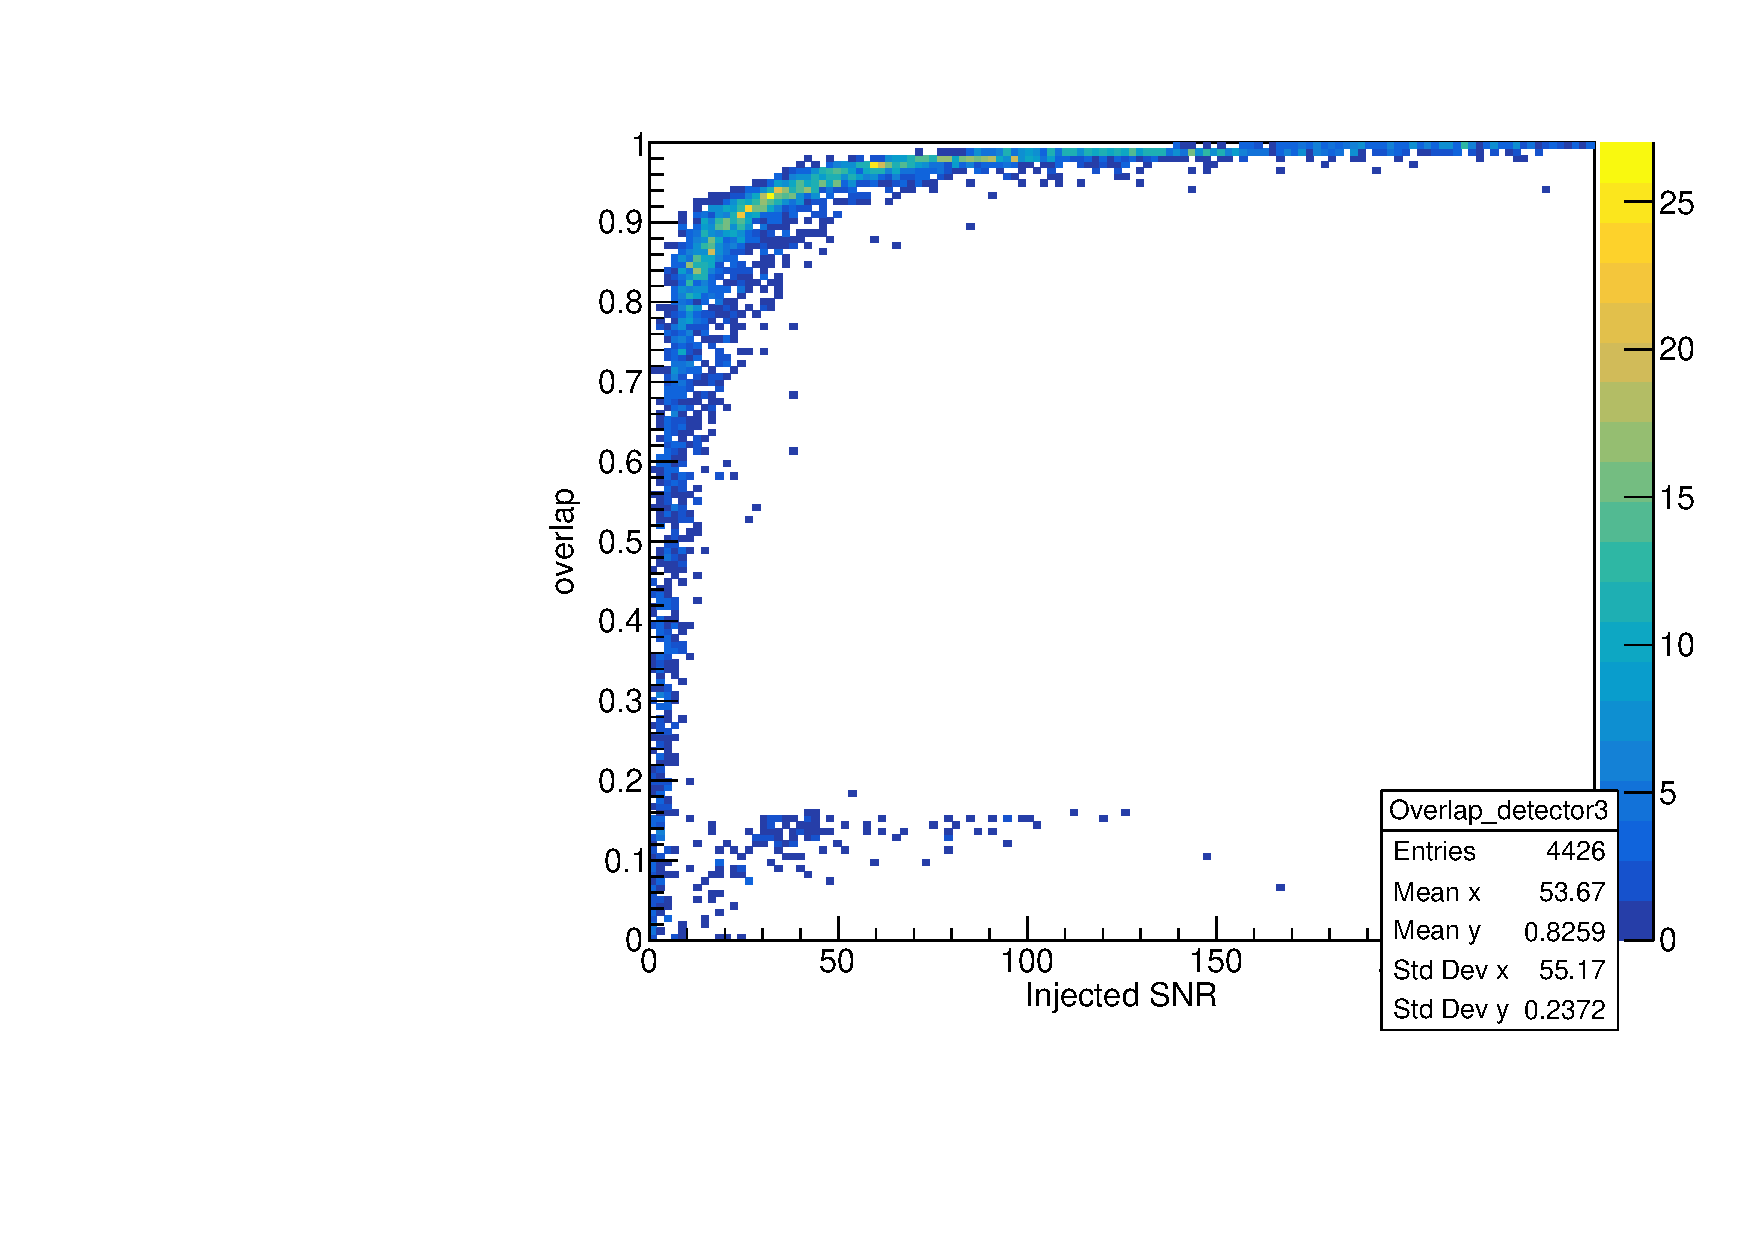
\includegraphics[width=.33\textwidth]{figures/Capitolo_4/OverlapDistributionDetector3APR4_q09.pdf}}
	\vspace{-5pt}
	\caption{Overlap per le due equazioni di stato}
	\label{fig:Overlap_SHT2_APR4}
	\vspace{-15pt}
\end{figure}
Il problema si ripresenta anche in questi grafici dove è possibile notare come vi sia per la EOS APR4 una certa quantità che non presenta l'andamento atteso. Si sono isolati gli eventi problematici e si è individuata la ragione della discrepanza: gli eventi che sporcano le distribuzioni sono tali perché vengono spezzati in fase di ricostruzione, c'è infatti una soglia in tempo e in frequenza dopo la quale due eccessi di potenza vengono spezzati in due eventi separati e può accadere, in particolare per la EOS APR4 che, come si è visto in \ref{subsection:APR4}, presenta un post merger a frequenze molto alte. Poiché la fase tra i due segnali, a bassa energia, non sempre viene ricostruita può accadere che il segnale venga spezzato in uno più energetico riguardante l'inspiral e uno meno, legato al post-merger. Questo si nota in particolar modo andando a confrontare la distribuzione delle frequenze minime e massime per le due EOS:
\begin{figure}[H]
	\vspace{-25pt}
	\centering
	\subfloat[][\emph{SHT2.0}]
	{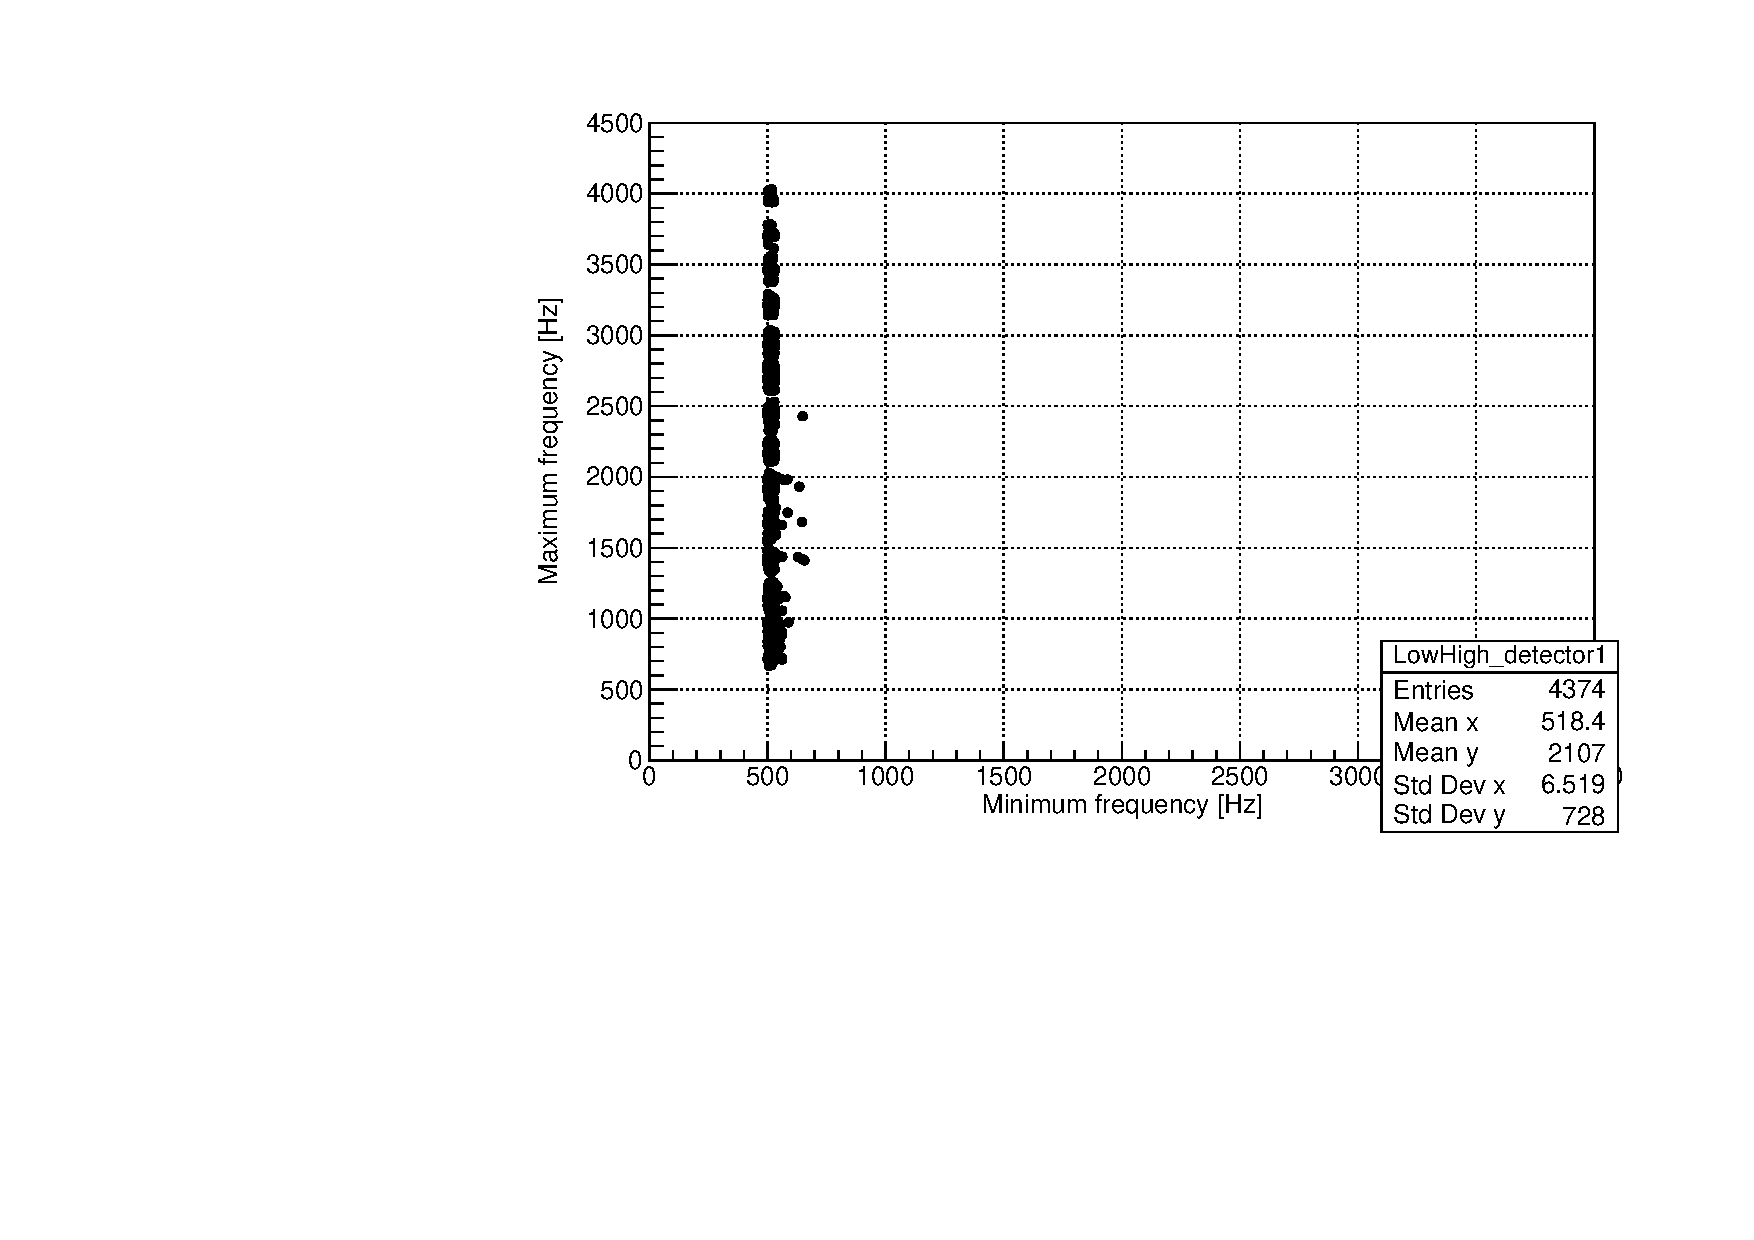
\includegraphics[width=.5\textwidth]{figures/Capitolo_4/FrequencyLHDistributionDetector1SHT2_0spin1.pdf}}% \quad\quad
	\subfloat[][\emph{APR4}]
	{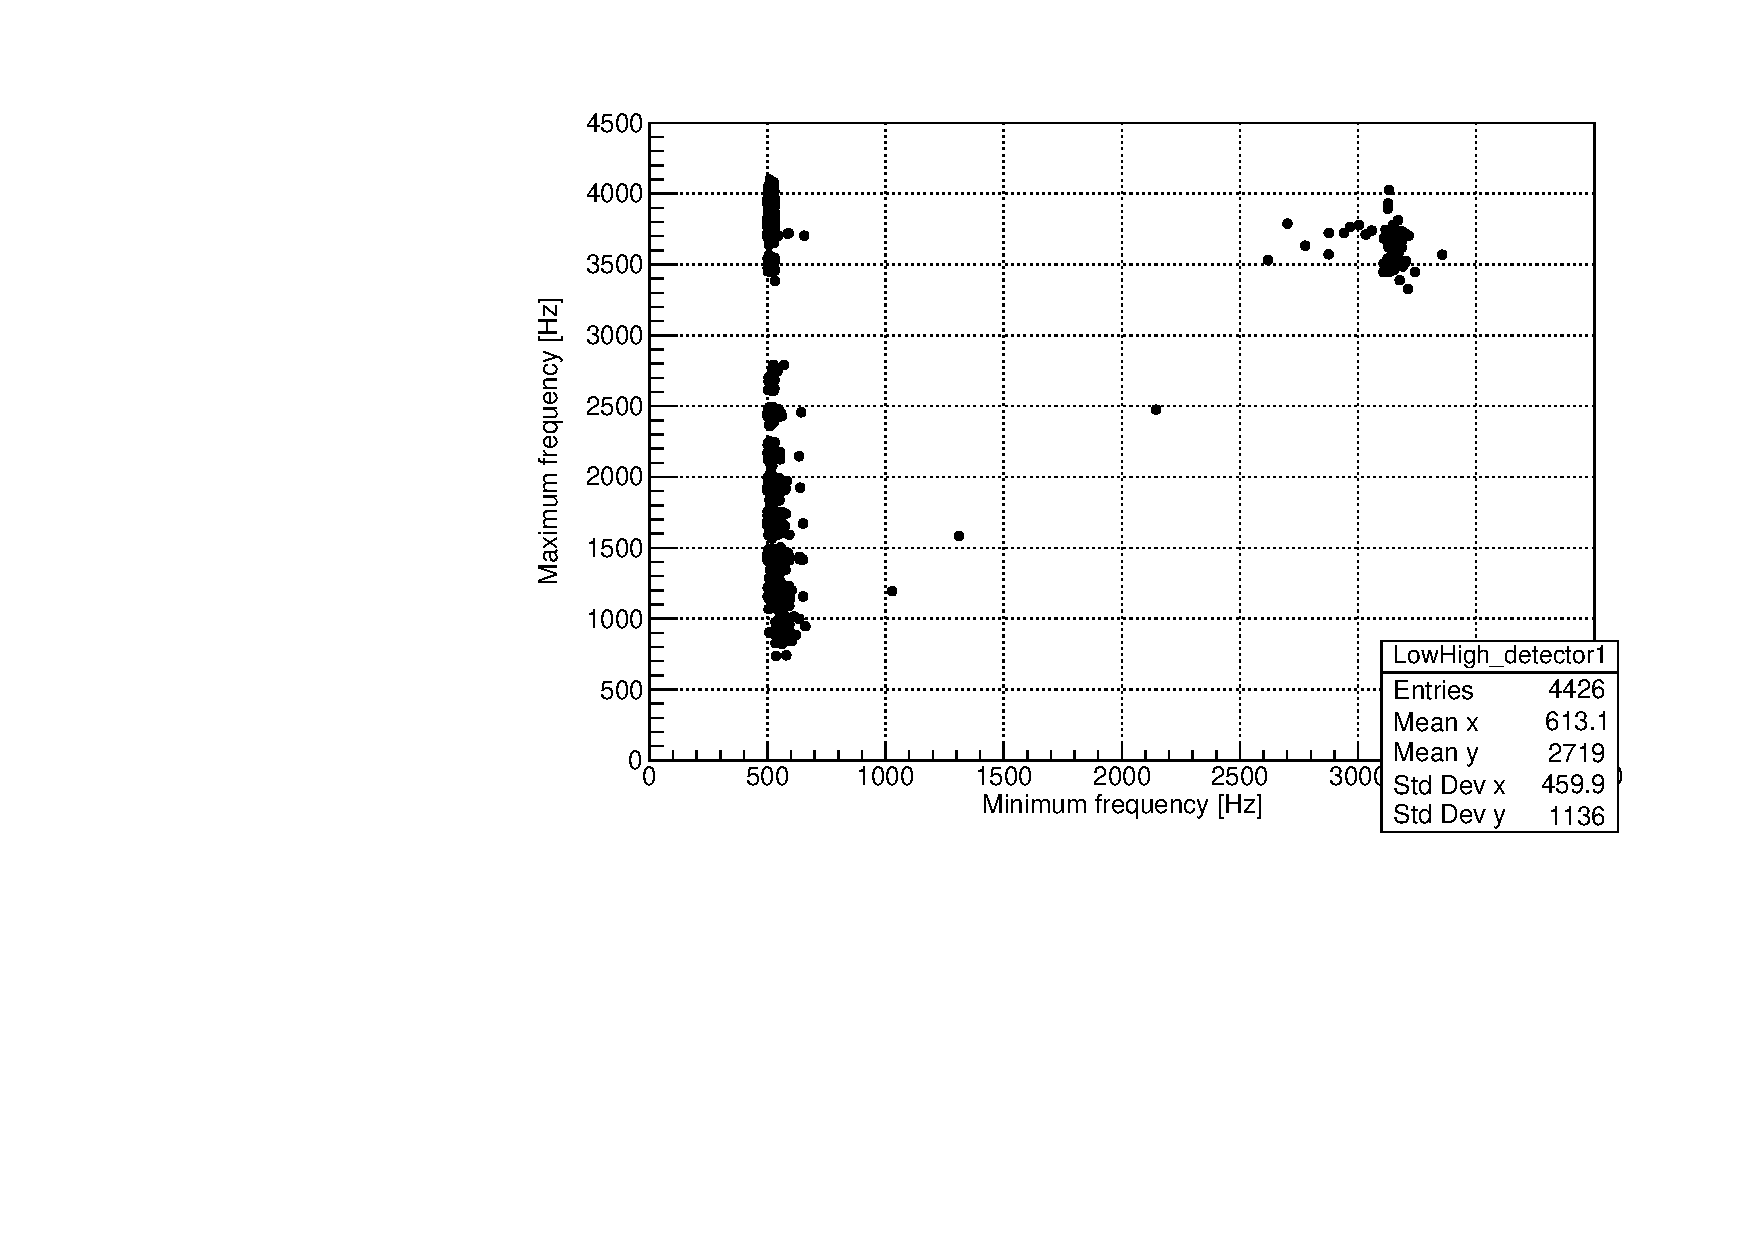
\includegraphics[width=.5\textwidth]{figures/Capitolo_4/FrequencyLHDistributionDetector1APR4_q09.pdf}}
	\vspace{-5pt}
	\caption{Distribuzione della frequenza massima e minima per le due EOS}
	\label{fig:Ffrequency_max_min}
	\vspace{-15pt}
\end{figure}
Si nota immediatamente per la EOS APR4 un cluster di eventi che presenta frequenza minima estremamente alta, incompatibile con l'andamento che assume un evento ricostruito in modo completo, che come descritto in precedenza dovrebbe avere l'andamento di un chirp, partendo da frequenza basse fino a un picco. Vengono quindi tagliati gli eventi ricostruiti nel solo post-merger. 
Ripetendo le precedenti analisi con il set di ricostruzioni tagliato si ottiene:
\begin{figure}[H]
	\vspace{-5pt}
	\centering
	\subfloat[][\emph{FIT}]
	{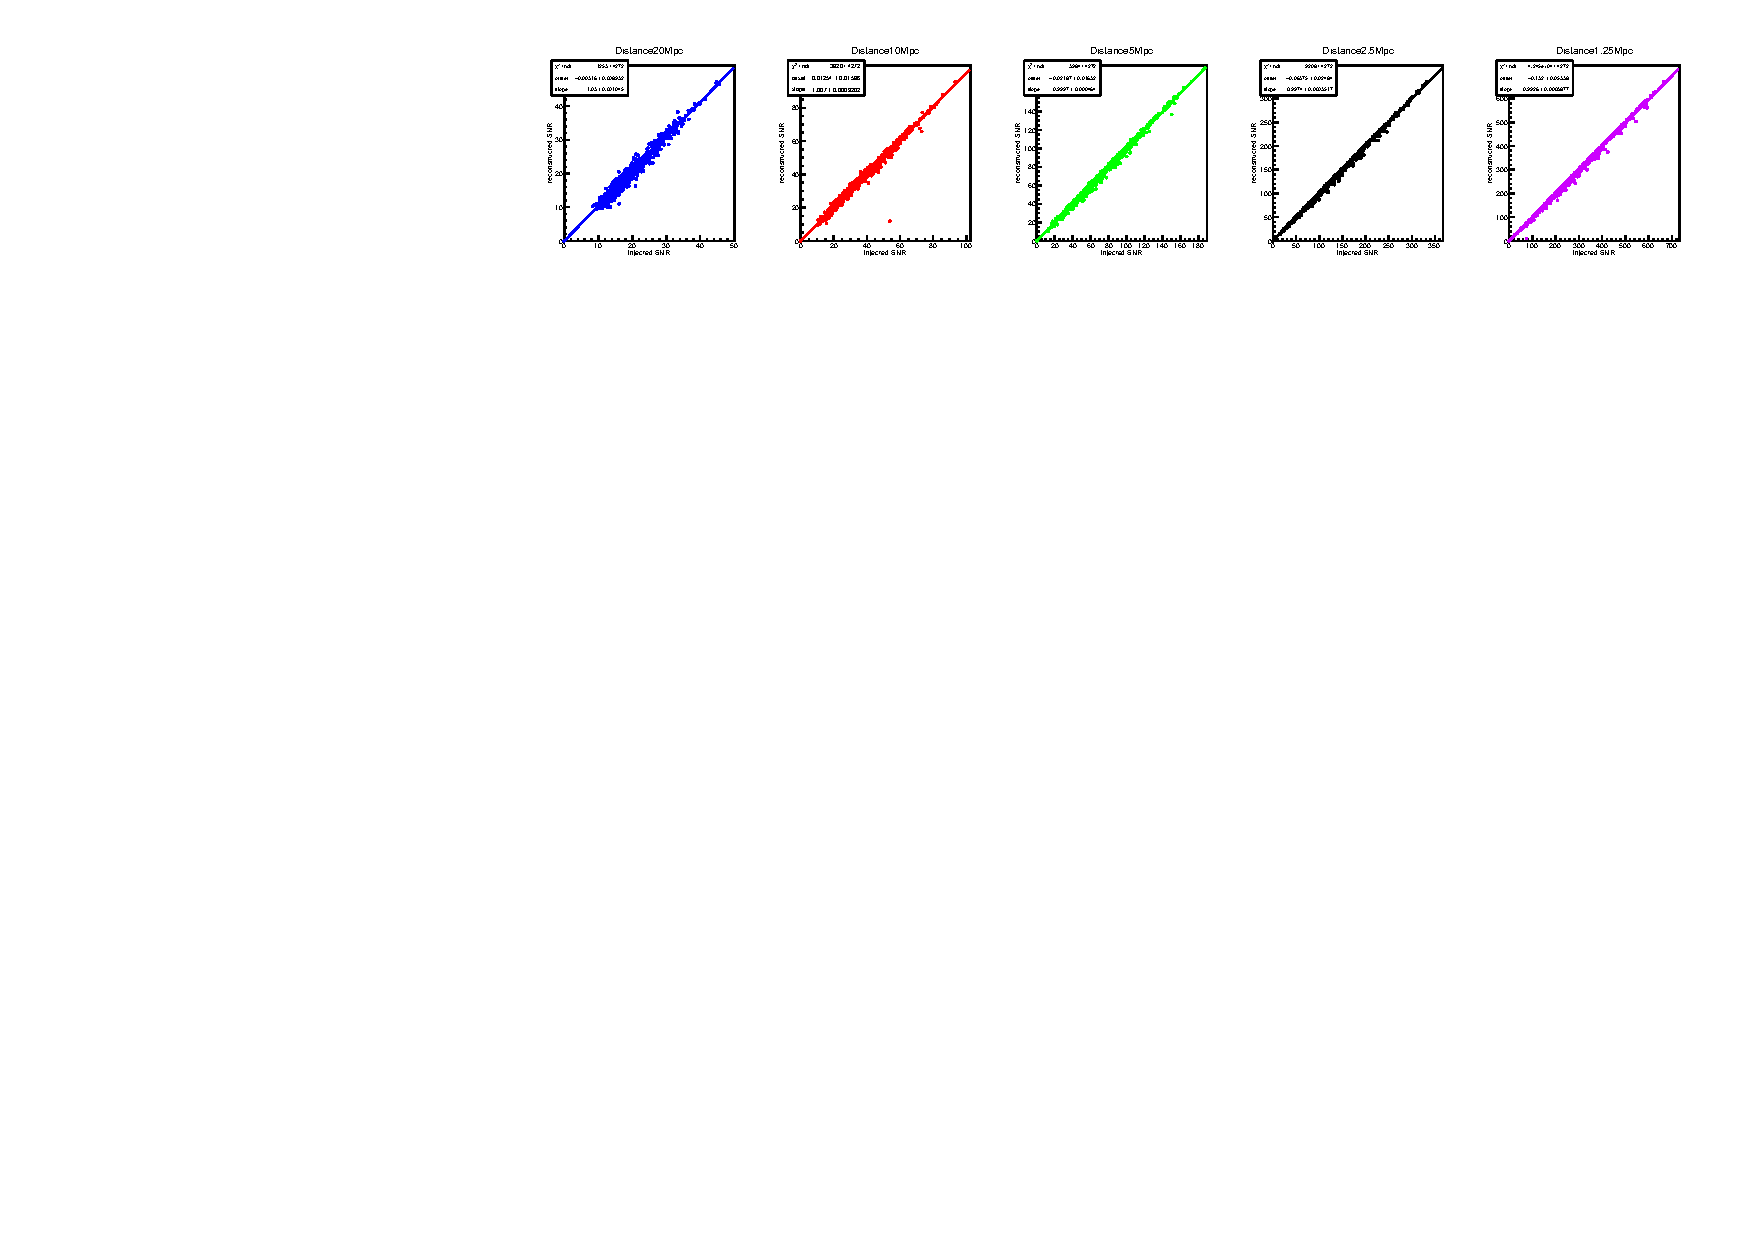
\includegraphics[width=1\textwidth]{figures/Capitolo_4/FITAPR4_q09_CUT.pdf}}\\
	\vspace{-10pt}
	\subfloat[][\emph{Energia residua per LIGO-Hanford}]
	{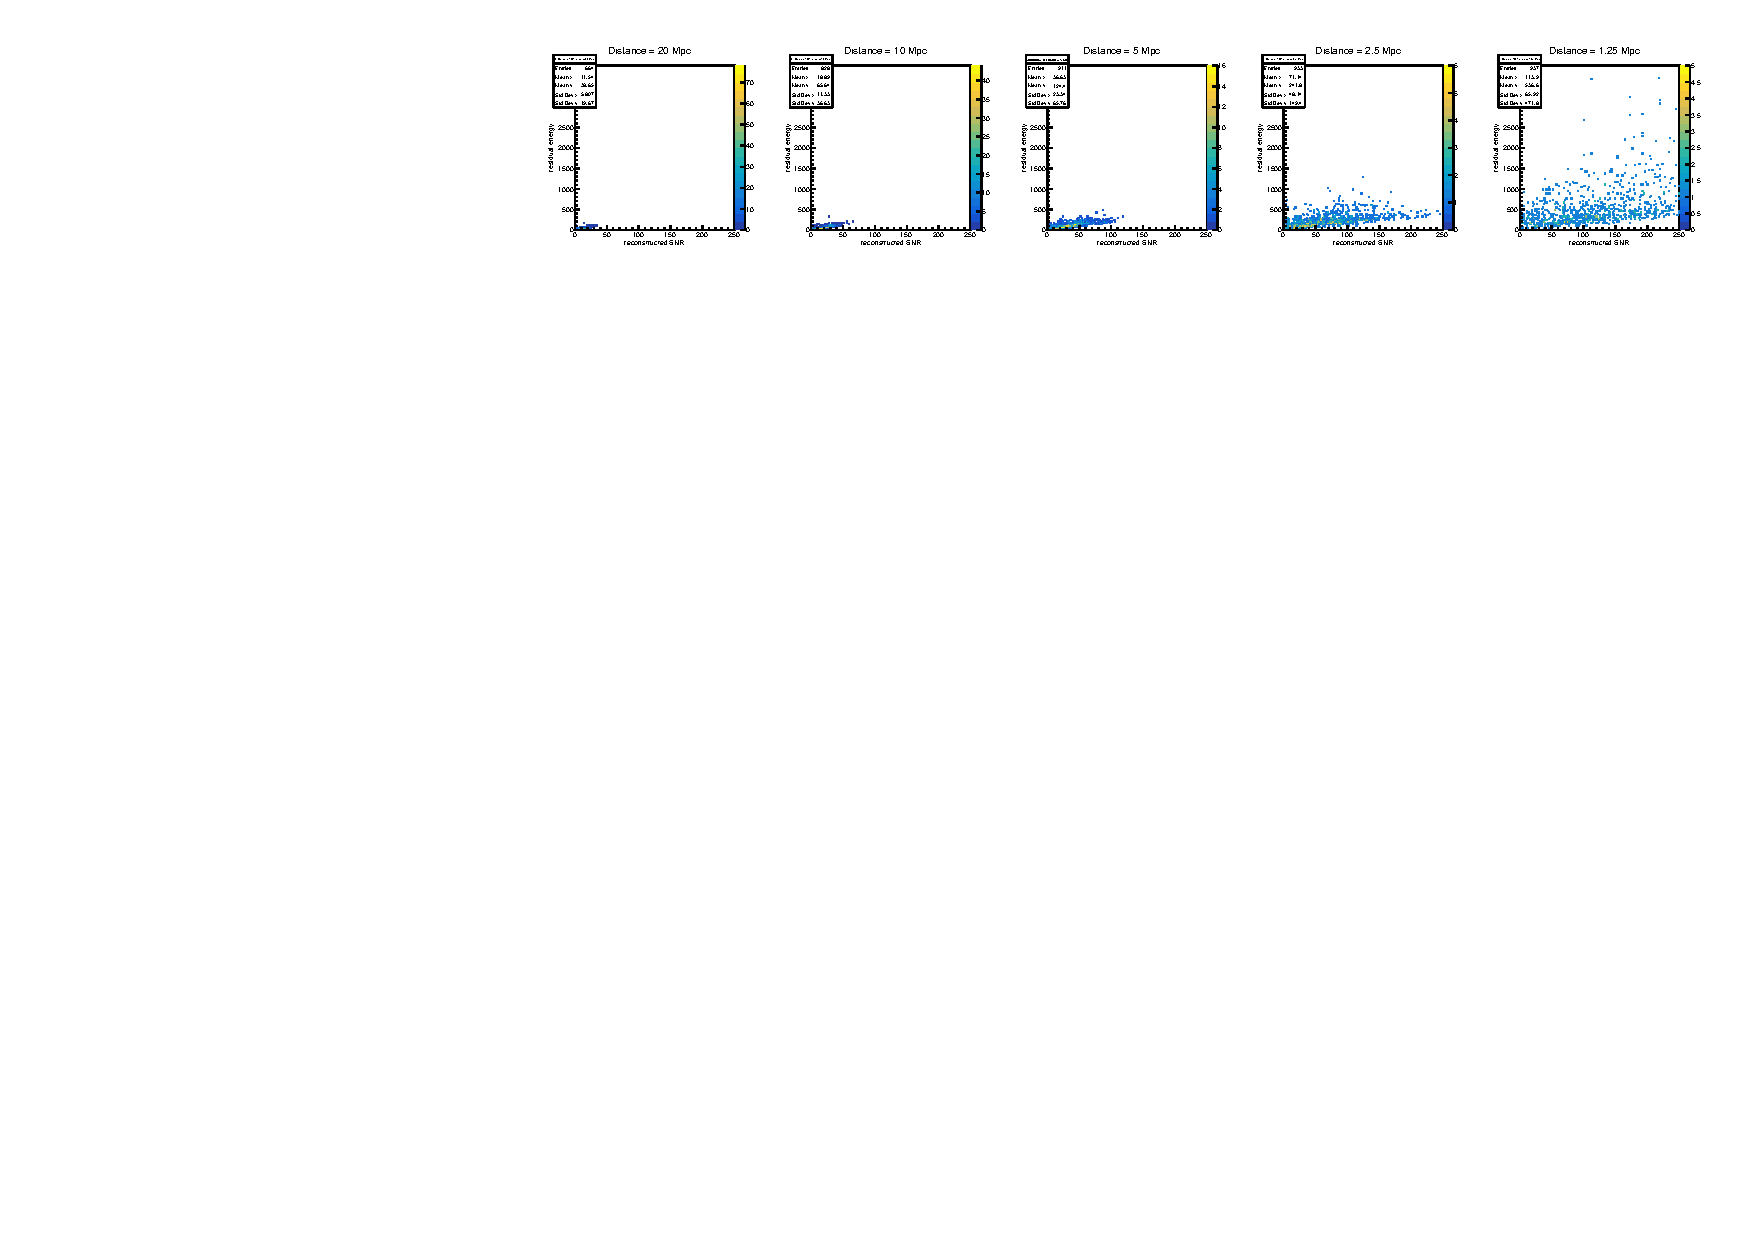
\includegraphics[width=1\textwidth]{figures/Capitolo_4/EnergyDistributionFactorDetector1APR4_q09_CUT.pdf}} \\
	\vspace{-10pt}
	\subfloat[][\emph{Overlap per LIGO-Hanford}]
	{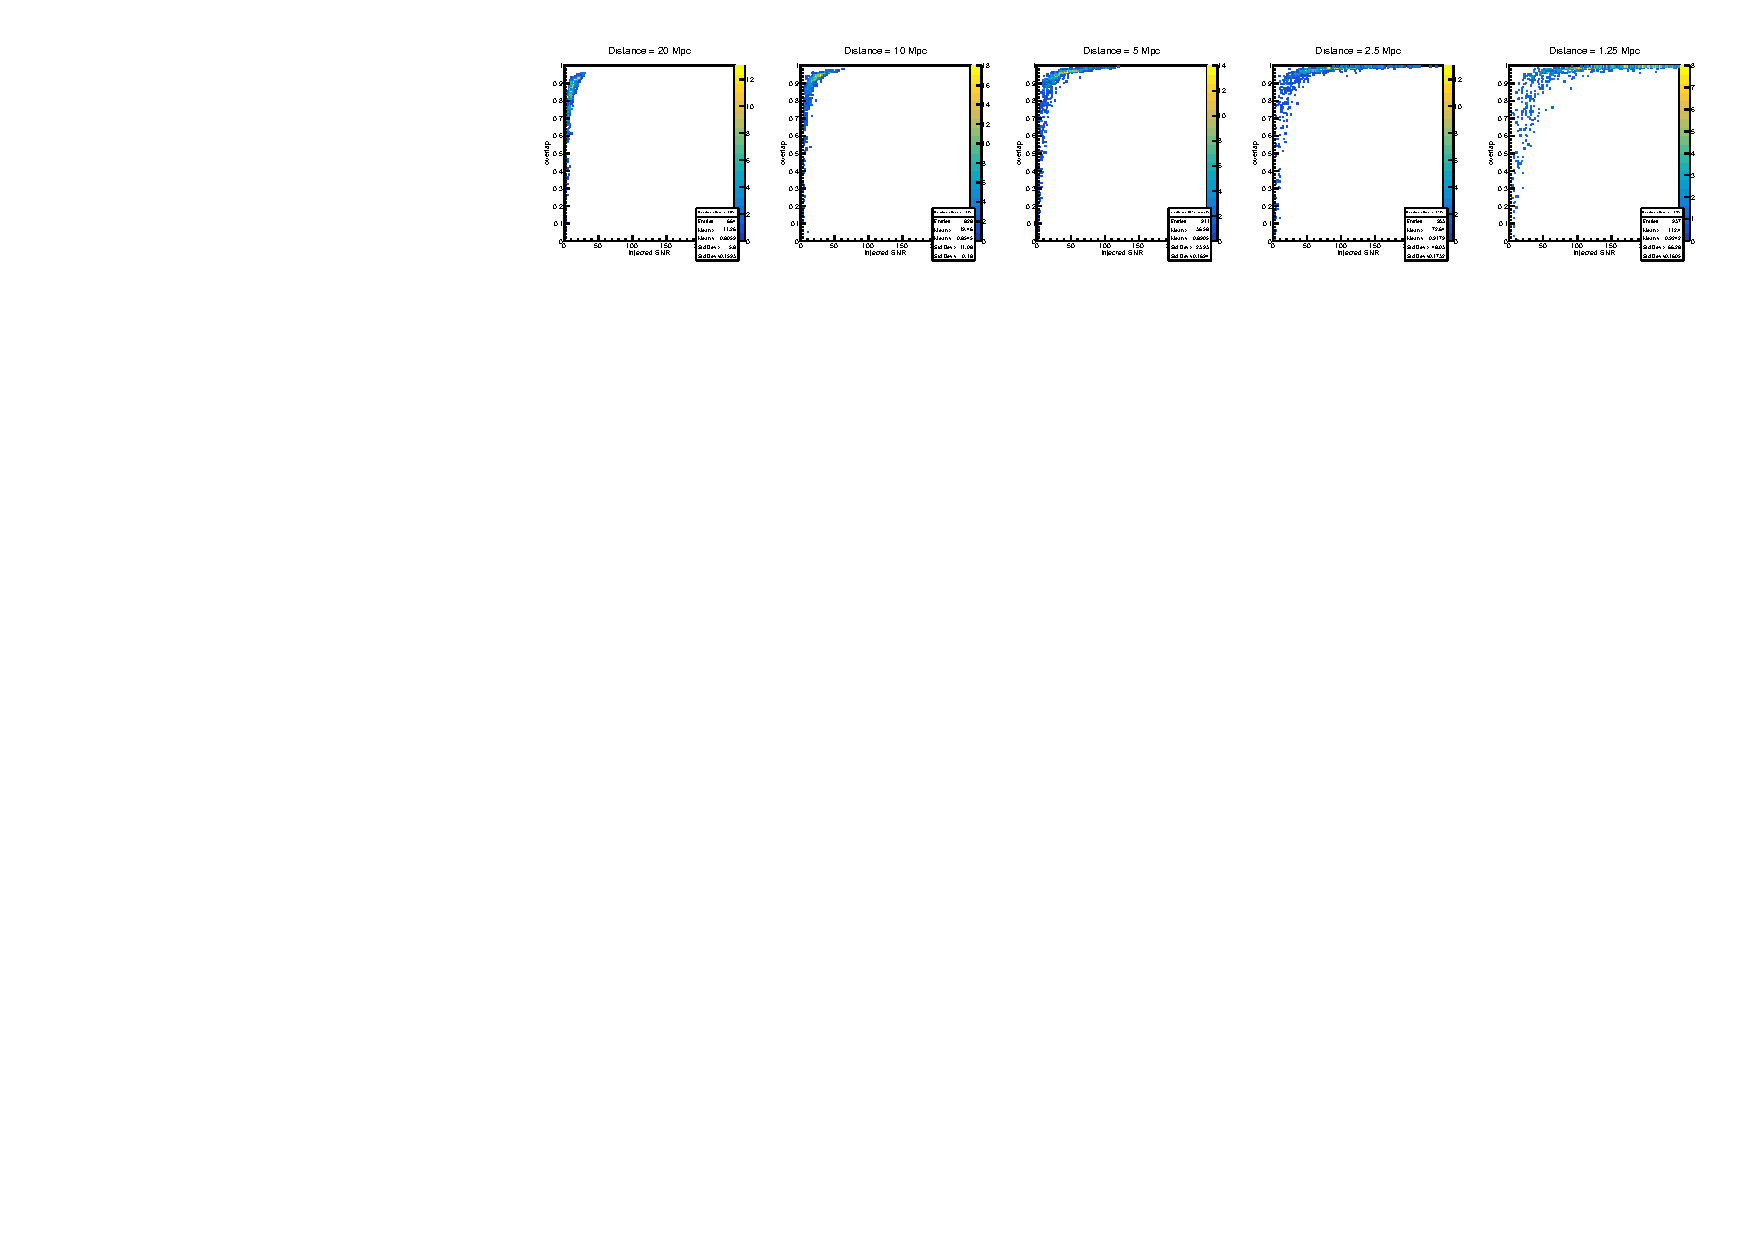
\includegraphics[width=1\textwidth]{figures/Capitolo_4/OverlapDistributionFactorDetector2APR4_q09_CUT.pdf}} 
	\vspace{-5pt}
	\caption{Analisi per APR4, fatta escludendo le ricostruzioni separate di uno stesso evento}
	\label{fig:apr4_cut}
	\vspace{-15pt}
\end{figure}
che presenta risultati non ottimali, come avviene per la EOS SHT2, ma comunque decisamente migliori rispetto ai dati non tagliati.

Gli overlap sono poi stati divisi in bin di SNR ricostruito di larghezza 10 per osservare la distribuzione con la quale i segnali sono ricostruiti 
%\begin{figure}[H]
%	\vspace{-15pt}
%	\centering
%	\subfloat[][\emph{SHT2.0}]
%	{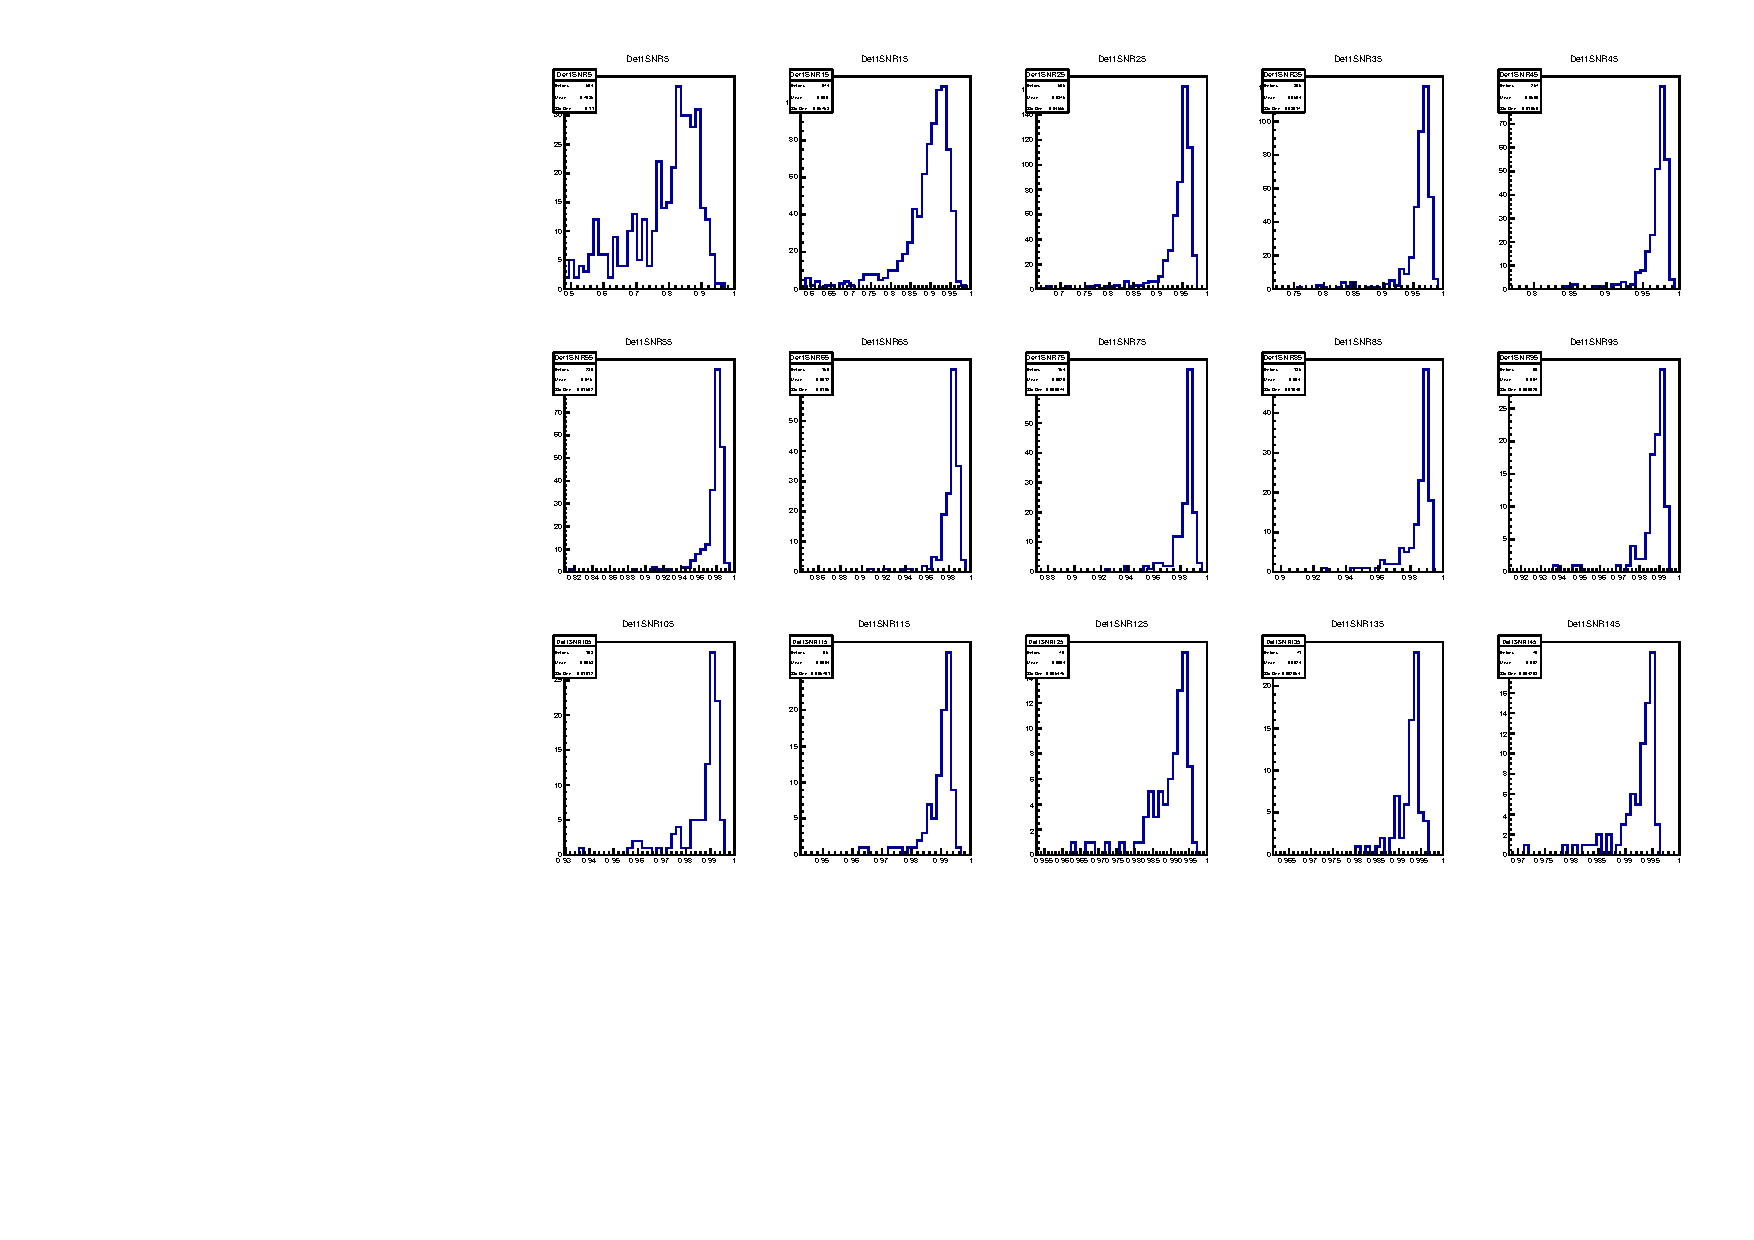
\includegraphics[width=.485\textwidth]{figures/Capitolo_4/OverlapDistributionsDetector1SHT2_0spin1.pdf}} \quad
%	\subfloat[][\emph{APR4}]
%	{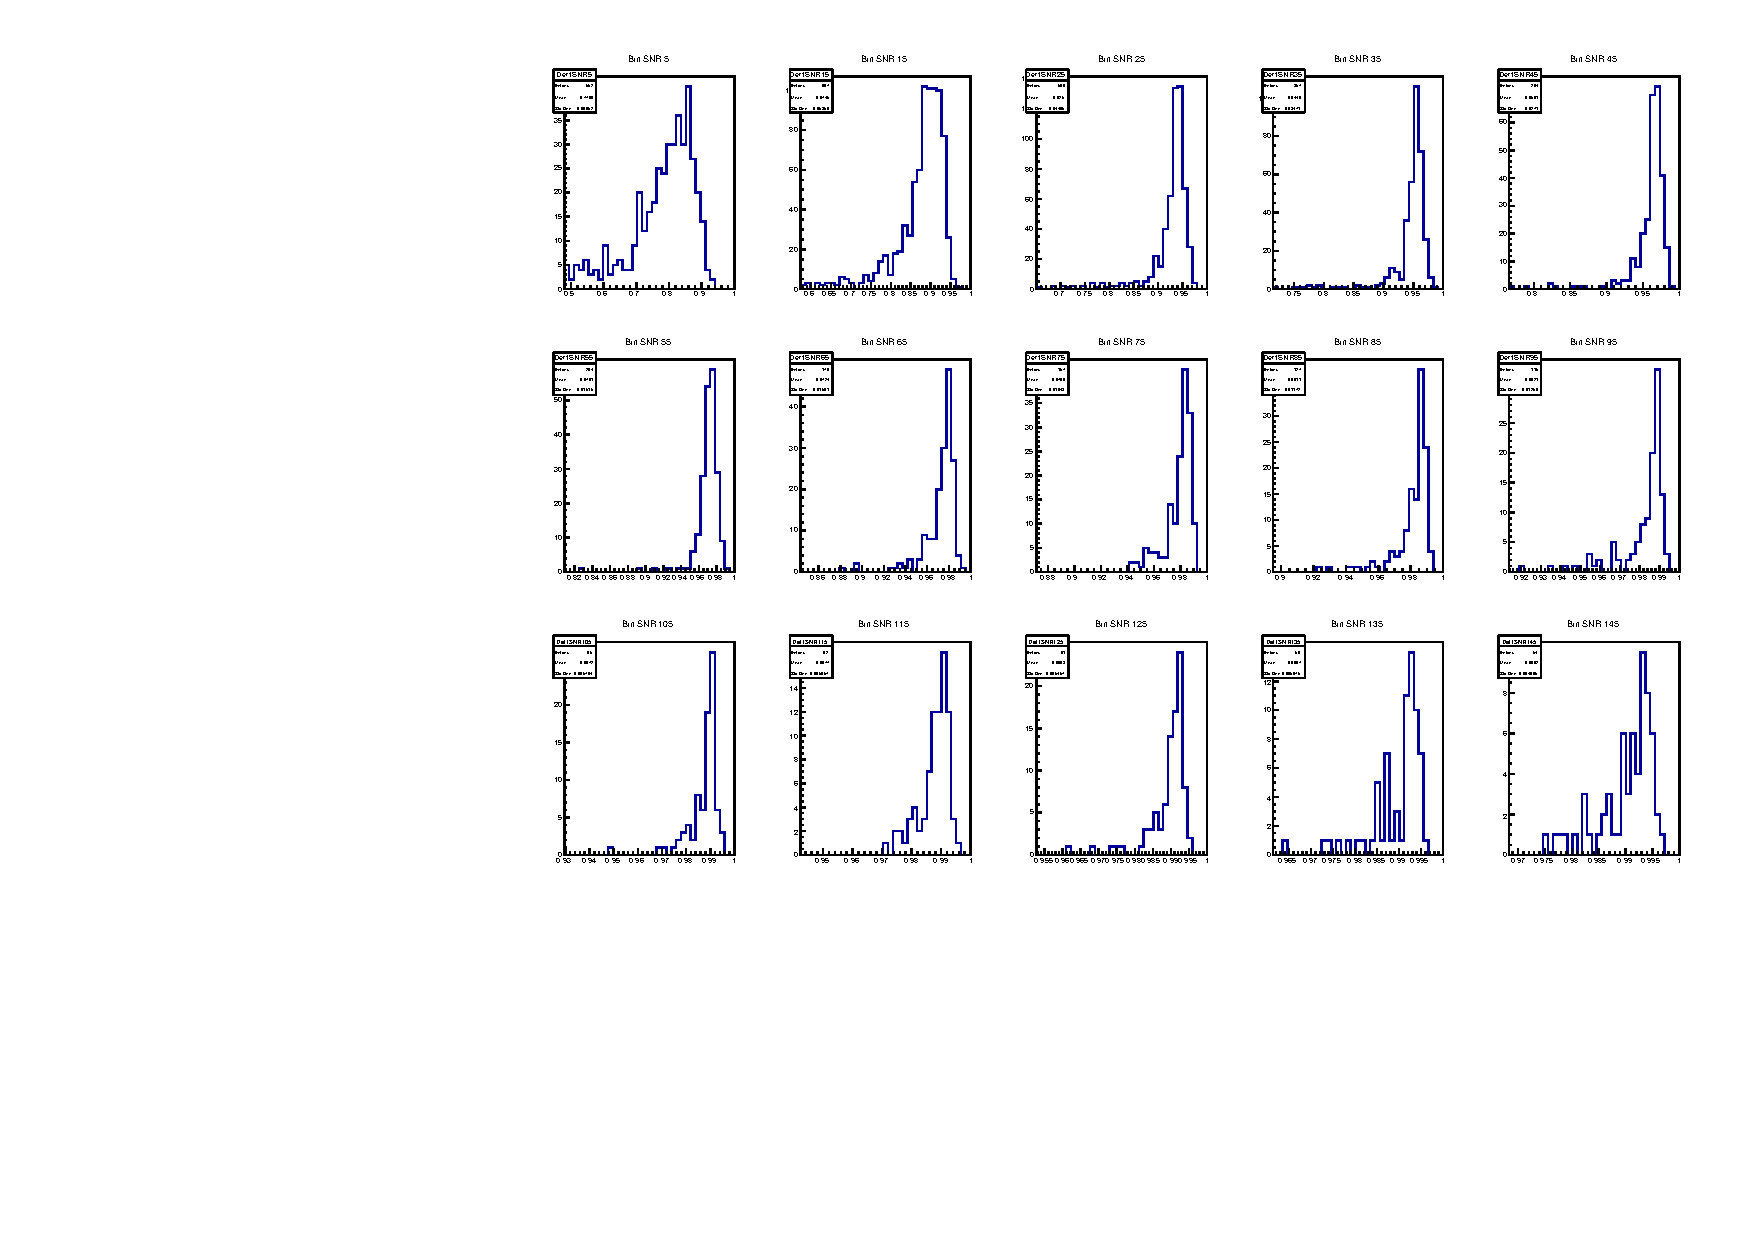
\includegraphics[width=.485\textwidth]{figures/Capitolo_4/OverlapDistributionsDetector1APR4_q09_CUT.pdf}}
%	\vspace{-5pt}
%	\caption{Distribuzione degli overlap per le due EOS}
%	\label{fig:Distributions_overlap}
%	\vspace{-15pt}
%\end{figure}
\begin{figure}[H]
	\vspace{-10pt}
	\centering
	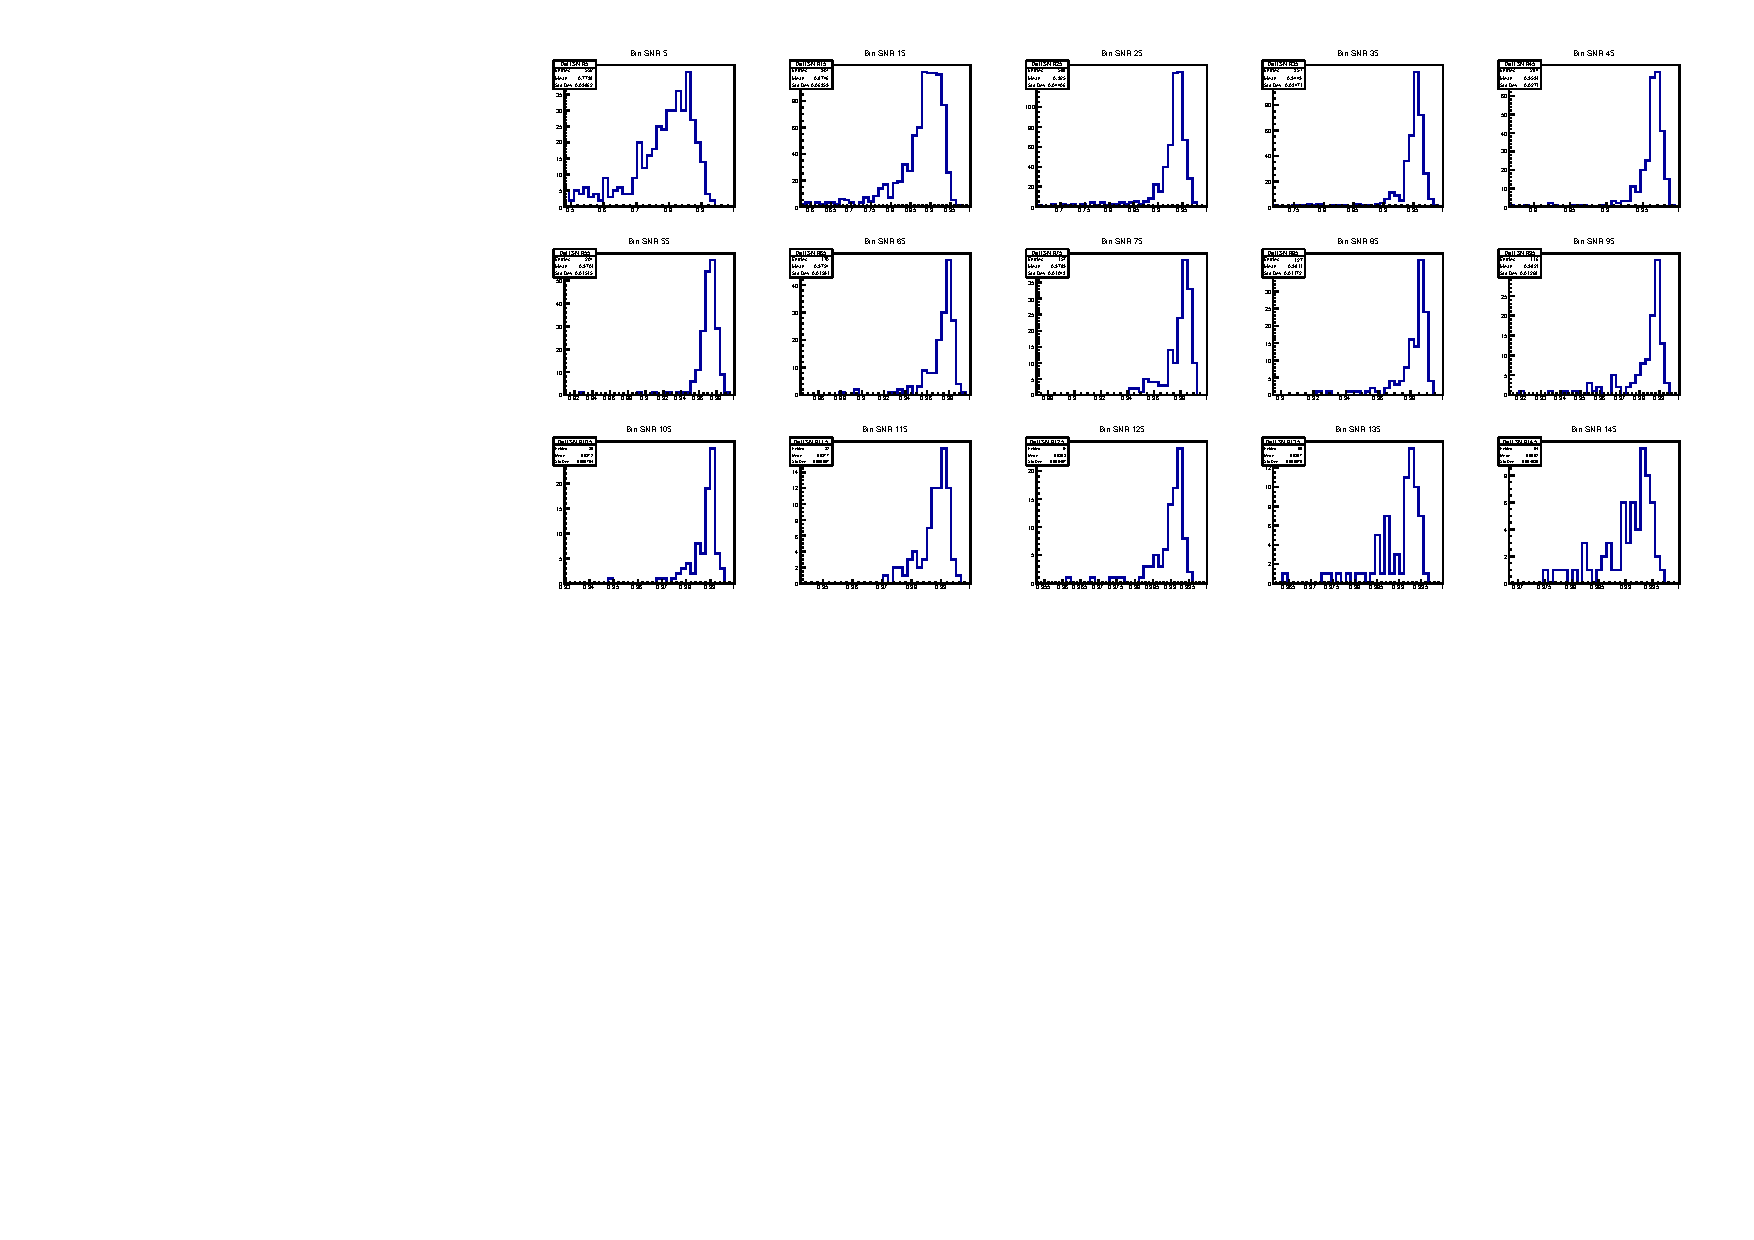
\includegraphics[width=1\textwidth]{figures/Capitolo_4/OverlapDistributionsDetector1APR4_q09_CUT_1.pdf}
	\vspace{-15pt}
	\caption{Distribuzione degli overlap per la EOS APR4 per il solo detector LIGO-Hanford, non si riportano, per ragioni di spazio, i grafici per gli altri detector e per l'altra EOS}
	\label{fig:Distributions_overlap}
	\vspace{-15pt}
\end{figure}
\begin{figure}[H]
	\vspace{-15pt}
	\centering
	\subfloat[][\emph{SHT2.0}]
	{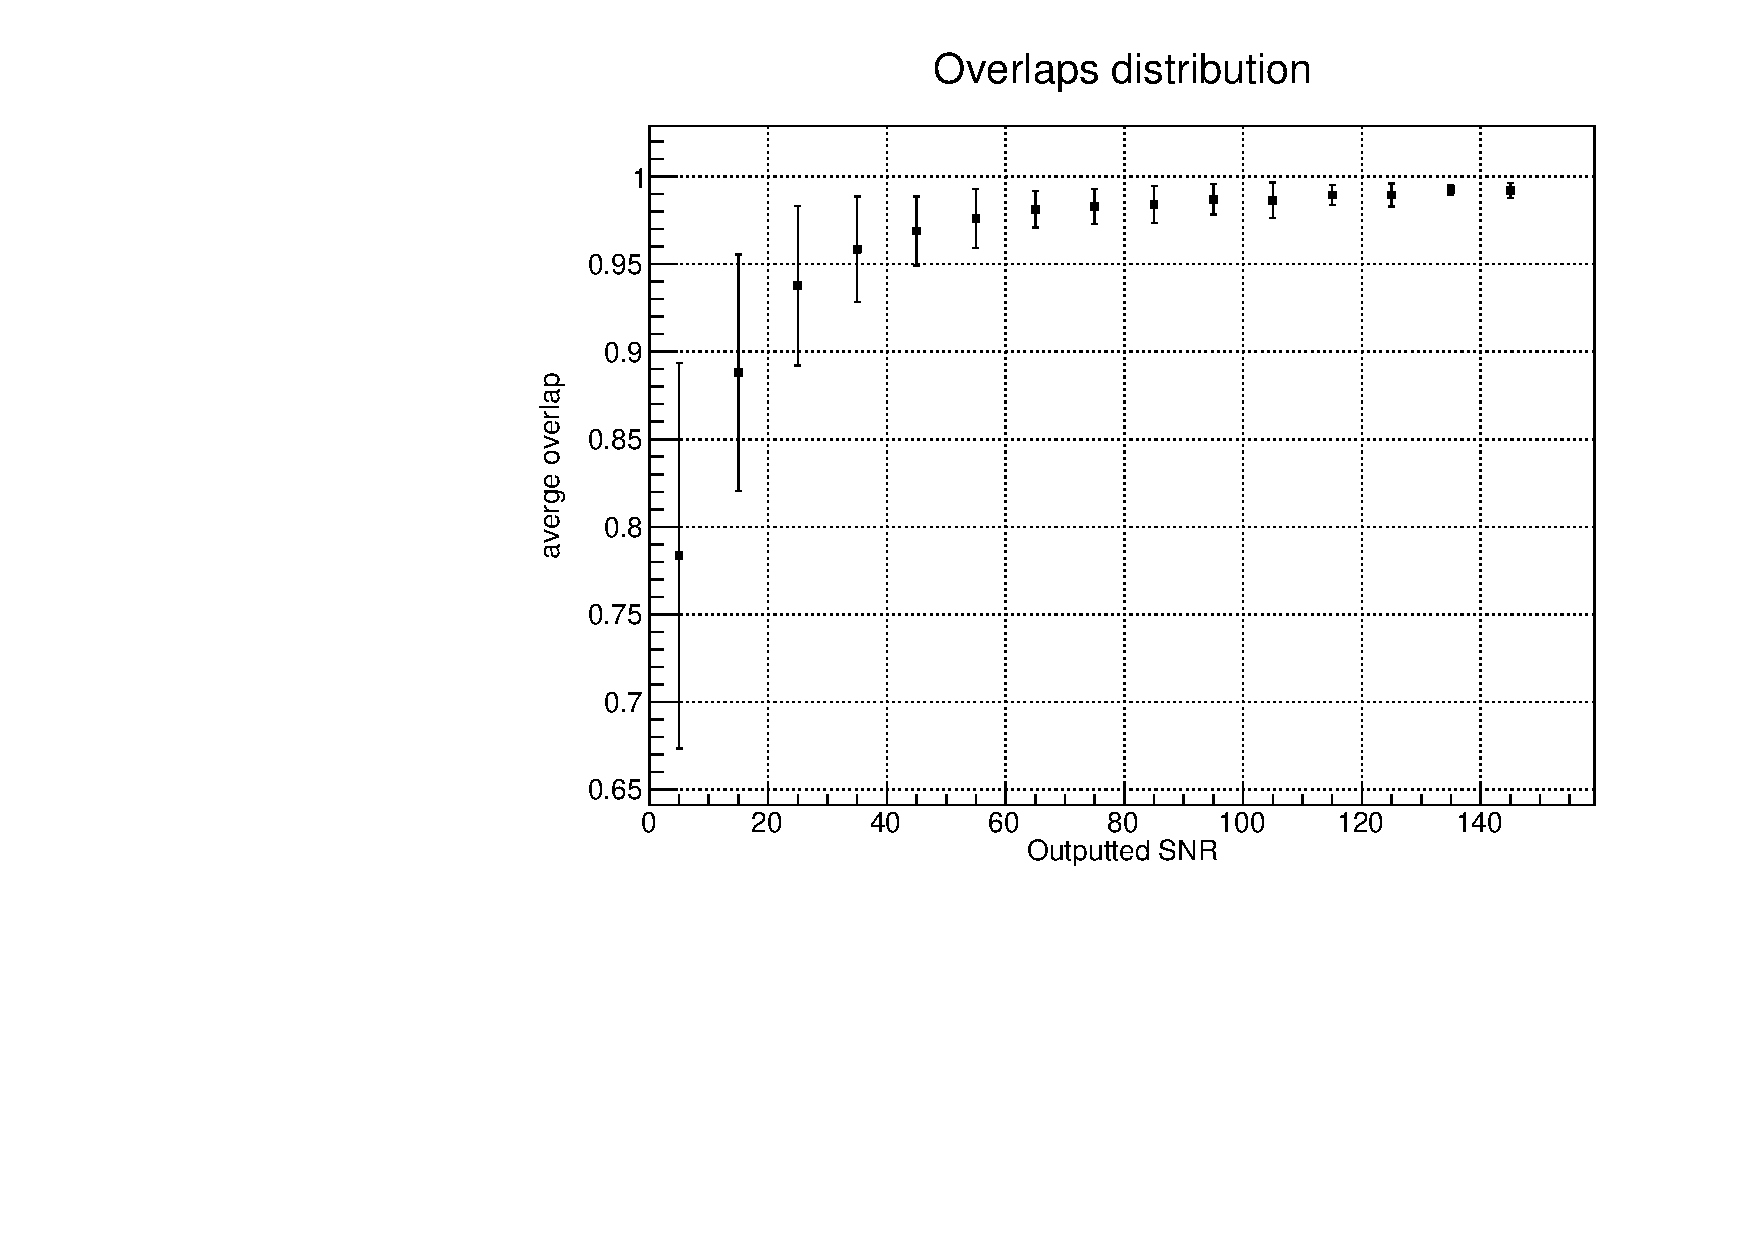
\includegraphics[width=.49\textwidth]{figures/Capitolo_4/Overlaps_GrapgDetector1SHT2_0spin1.pdf}} \hspace{0.5pt}
	\subfloat[][\emph{APR4}]
	{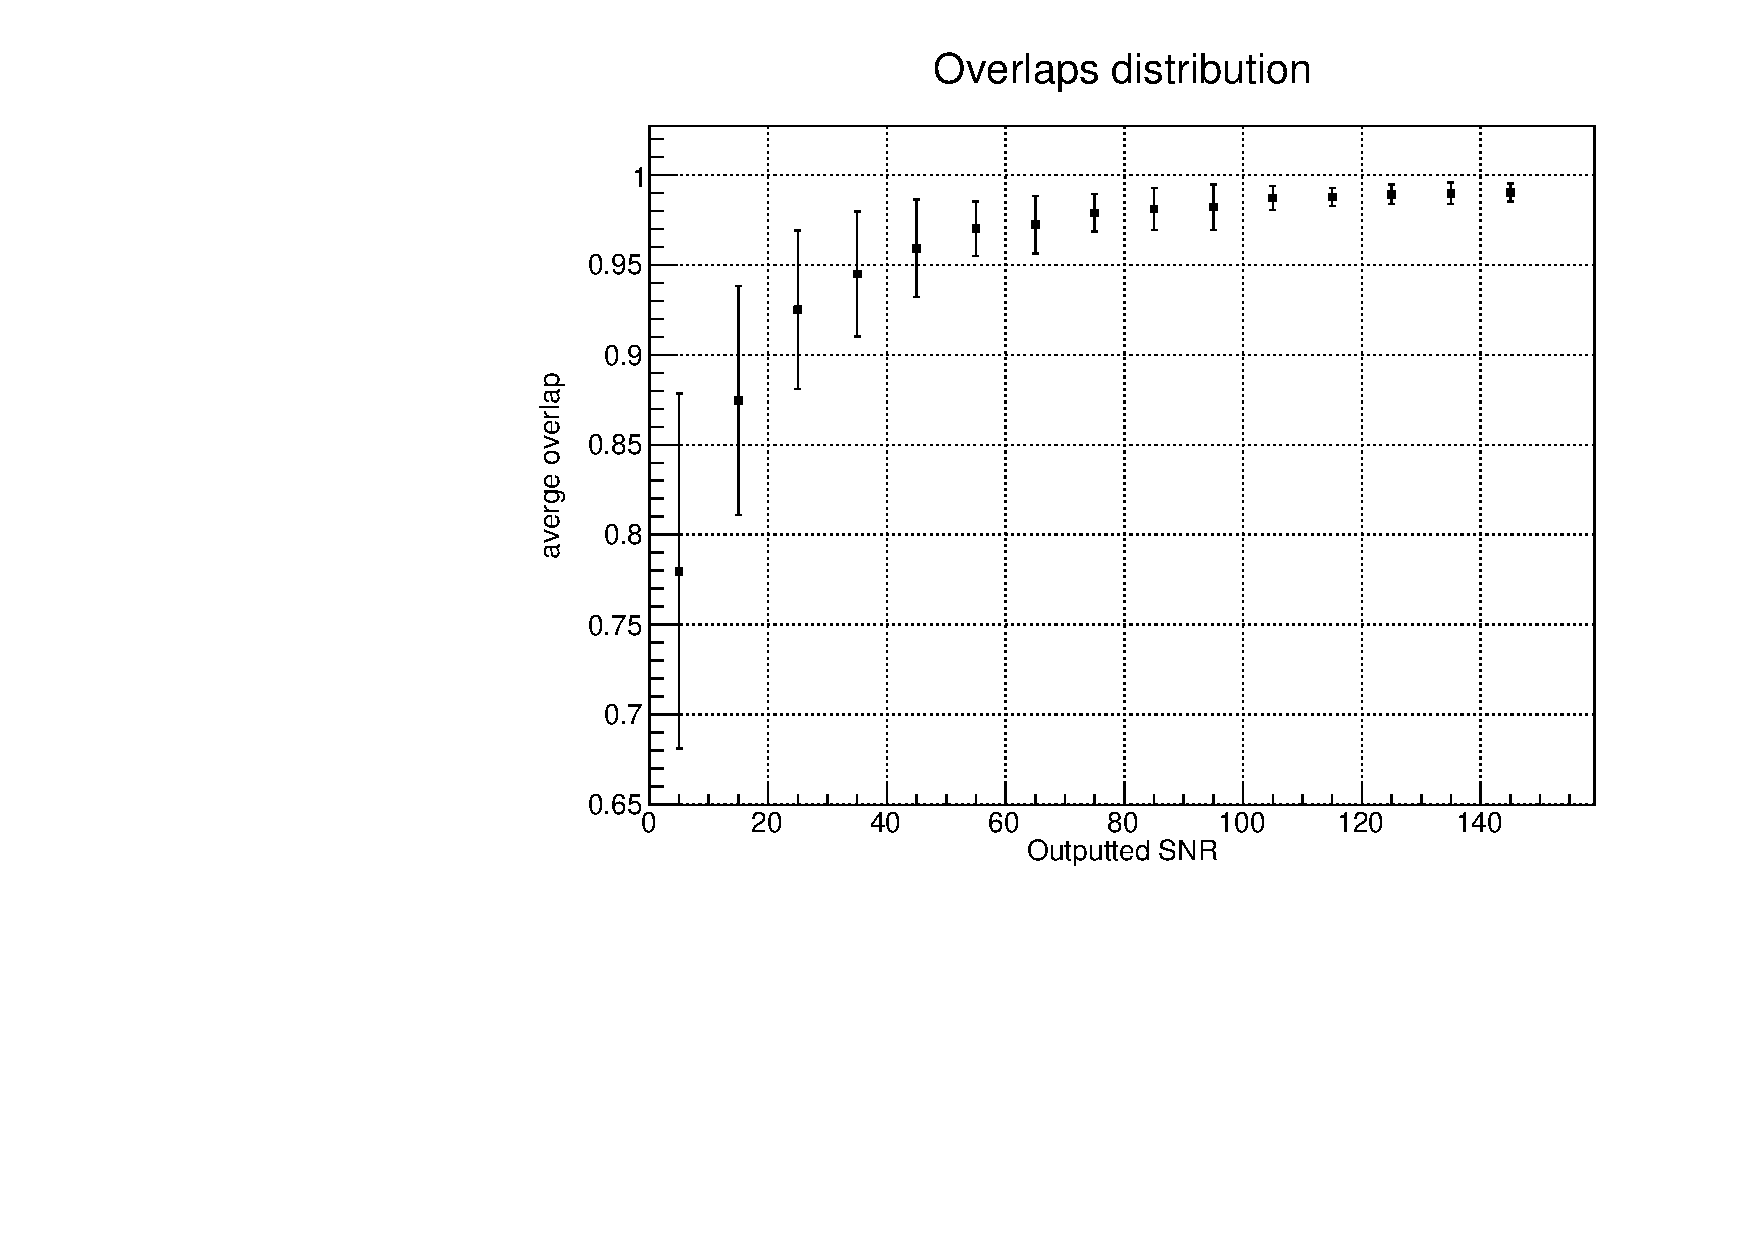
\includegraphics[width=.49\textwidth]{figures/Capitolo_4/Overlaps_GrapgDetector1APR4_q09_CUT.pdf}}
	\vspace{-5pt}
	\caption{Distribuzione degli overlap per le due EOS}
	\label{fig:Overlap_distribution}
	\vspace{-15pt}
\end{figure}

\section{Ricerca frequenza post-merger}

Per valutare la frequenza della post-coalescenza l'analisi viene fatta su un campione di $\smallsim$ 500 eventi simulati. 

%\lipsum[8]
%\lipsum[9]